\section{One-dimensional Chain}
\label{sec:1d-chain}

The analytical solution of the \acs{1D} Hubbard model at half filling indicates that the ground state is antiferromagnetic \cite{lieb_absence_1968}.
To build a physical picture of the Hubbard chain, start by considering the $\frac{U}{t} \gg 1$ limit. 
Then, the Hubbard model can be replaced by an effective atomic Heisenberg model defined in the Hilbert subspace with one electron per site, and \ac{AF} order sets in.
In the Hubbard model, at zero temperature, it is found that upon decreasing $U$, the system is not only \acs{AF} for large $U$, but remains an \acs{AF} \emph{insulator} down to $U \rightarrow 0$, becoming a \emph{conductor} and losing \acs{AF} order only at $U = 0$.
Thus, for high enough $\beta = t / T$, we expect to see signs of \acs{AF} order for all $0 < U < \infty$.
Upon decreasing $\beta$, thermal fluctuations tend to completely destroy long range order.
Conversely, as $\beta$ is increased, we expect to see a divergence in $\chi$, corresponding to a phase transition to the antiferromagnetic ground state.
We identify it by measuring both the equal-time and time-displaced spin-spin correlation functions, $\left\langle S^z_i  S^z_j \right\rangle$ and $\left\langle S^z_i (\tau) S^z_j (0) \right\rangle$ with Monte Carlo.
Fourier transforming as per Eqs.(\ref{eq:S(q)},\ref{eq:chi(q)}), we obtain a peak at $q = \pi$ in the magnetic structure factor $S ( q ) $, and in the magnetic susceptibility $\chi (q)$.
Both peaks increase in magnitude as temperature is decreased, and in fact, within statistical uncertainty, the \say{staggered} susceptibility $\chi (\pi)$ appears to diverge very near $T_c = 0$.
Contrastingly, the $q = 0$ components of both the structure factor and the susceptibility go to zero as the temperature is decreased, indicating  no sign of ferromagnetic ordering in the ground state.
\begin{figure}[H]\label{fig:corr_FT}
\hspace{0.2cm}
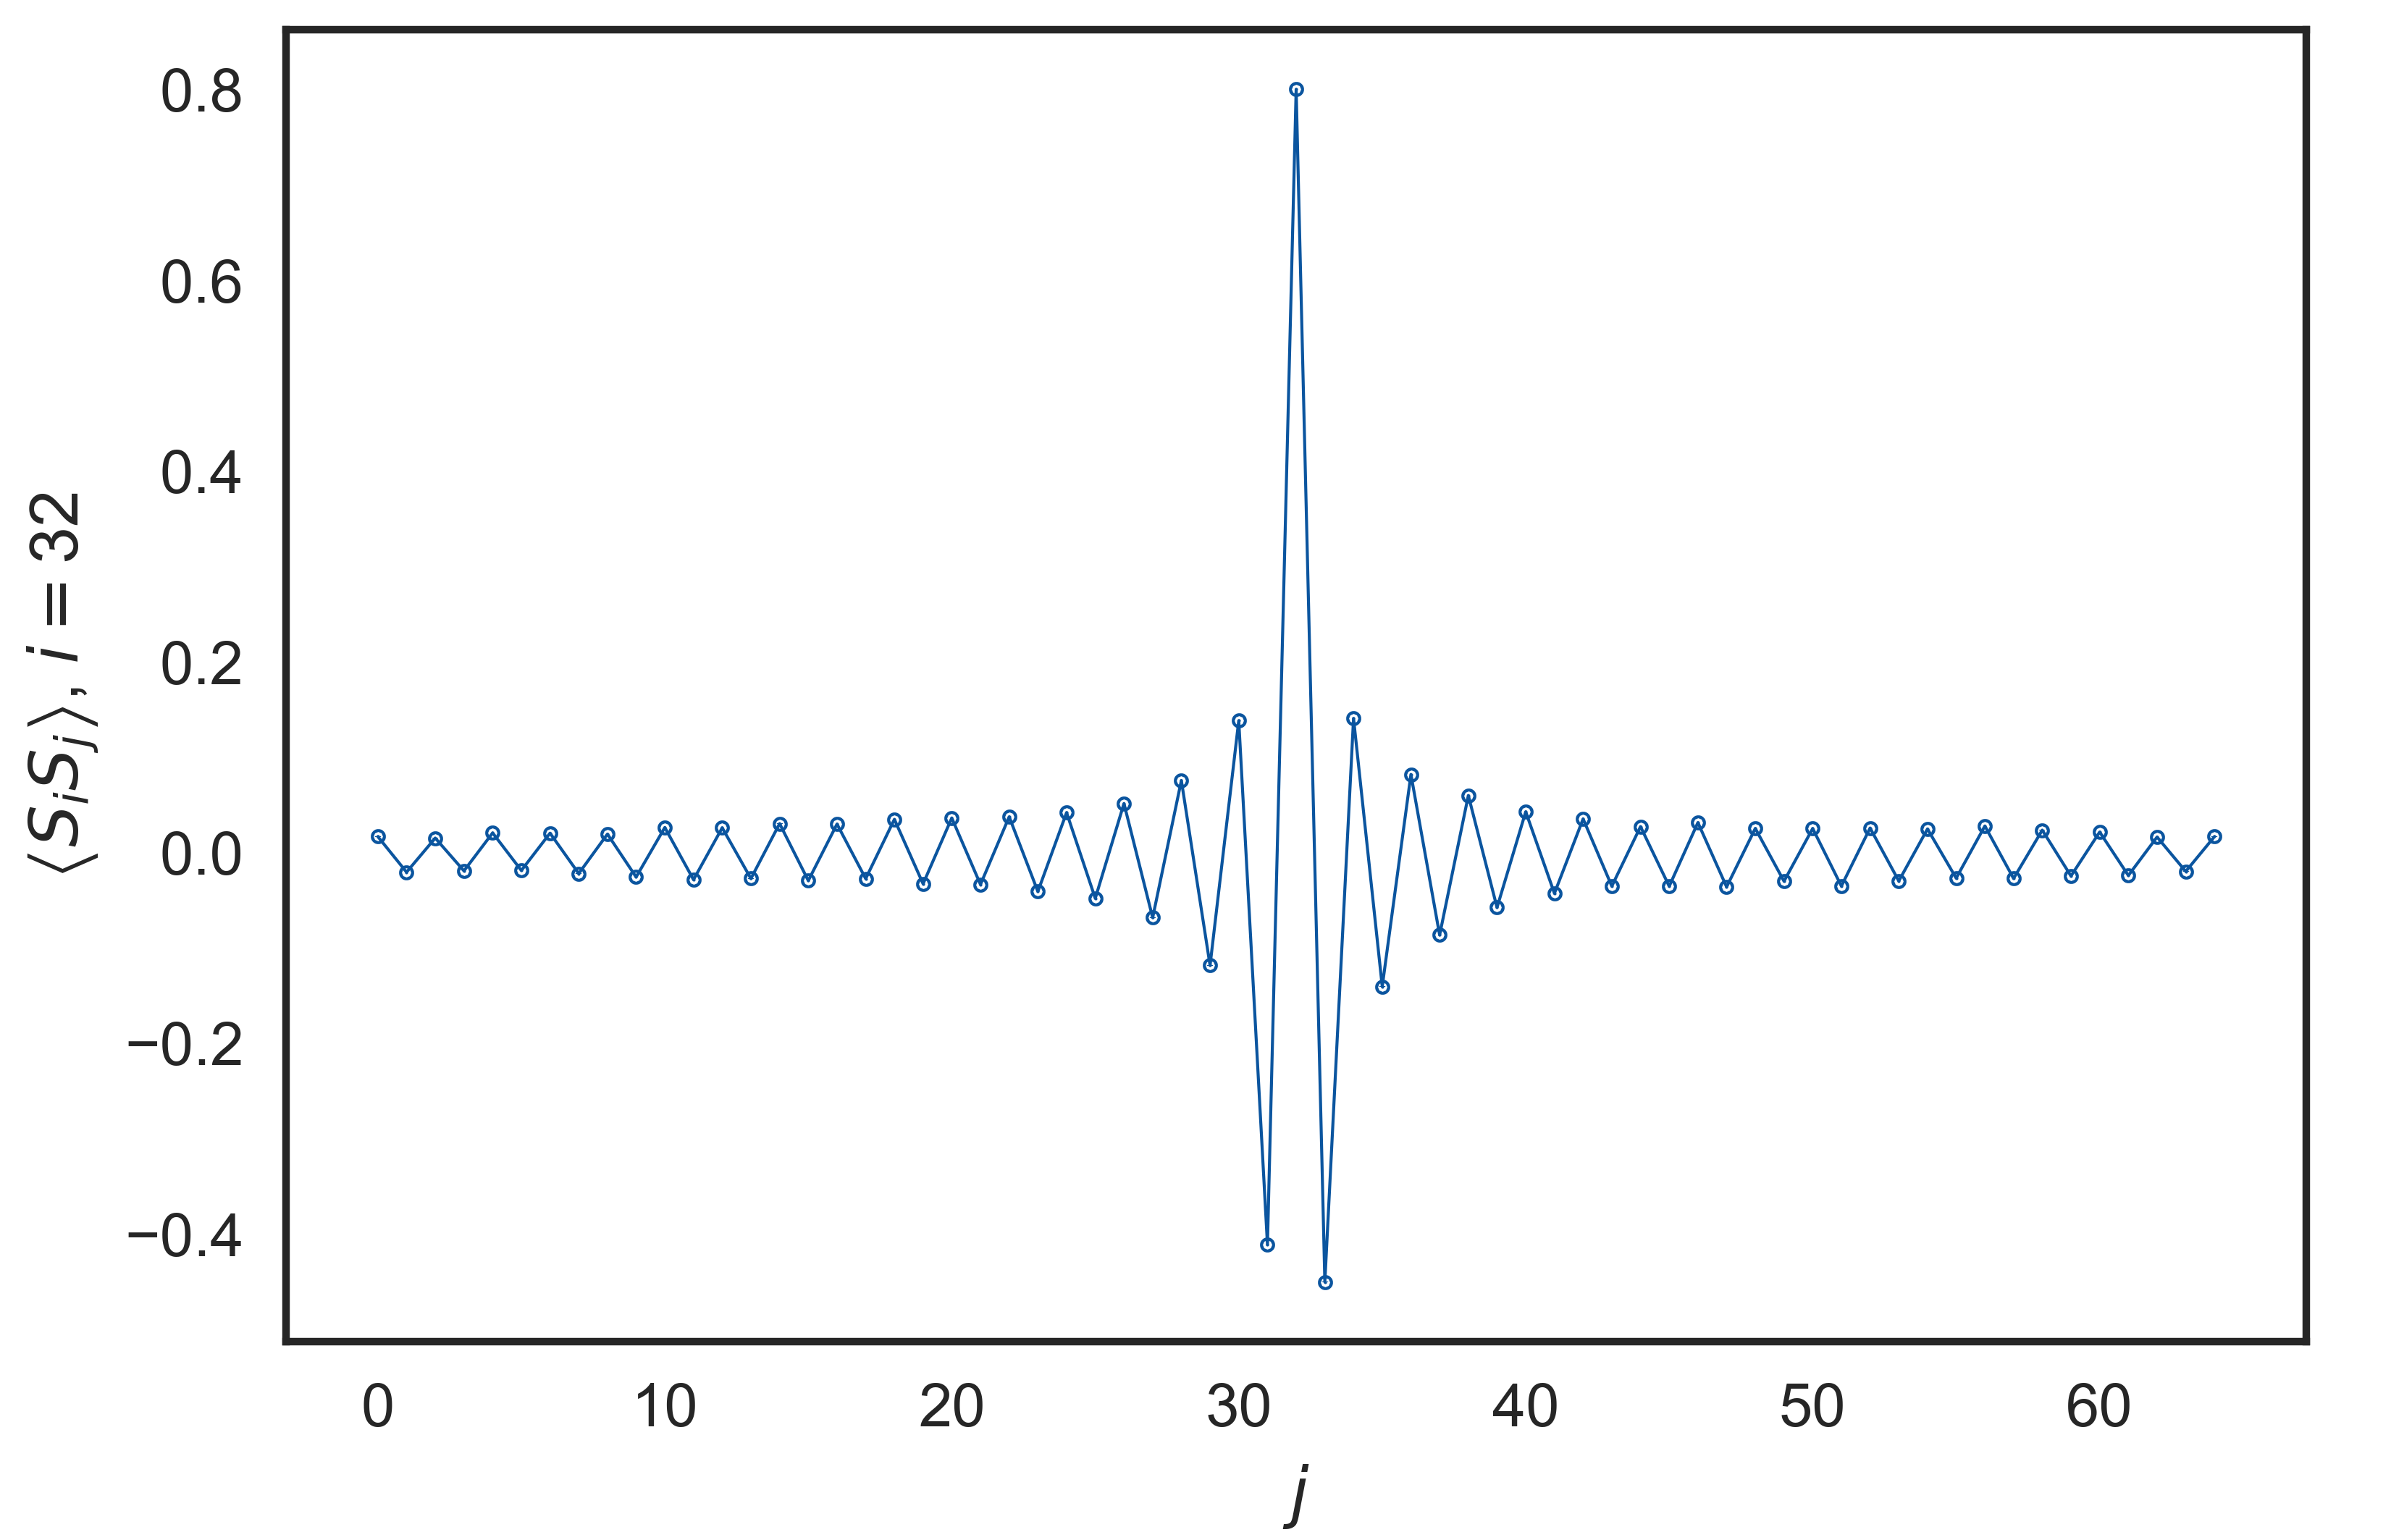
\includegraphics[scale=0.53]{Applications/magCorr.png}
\hspace{0.7cm}
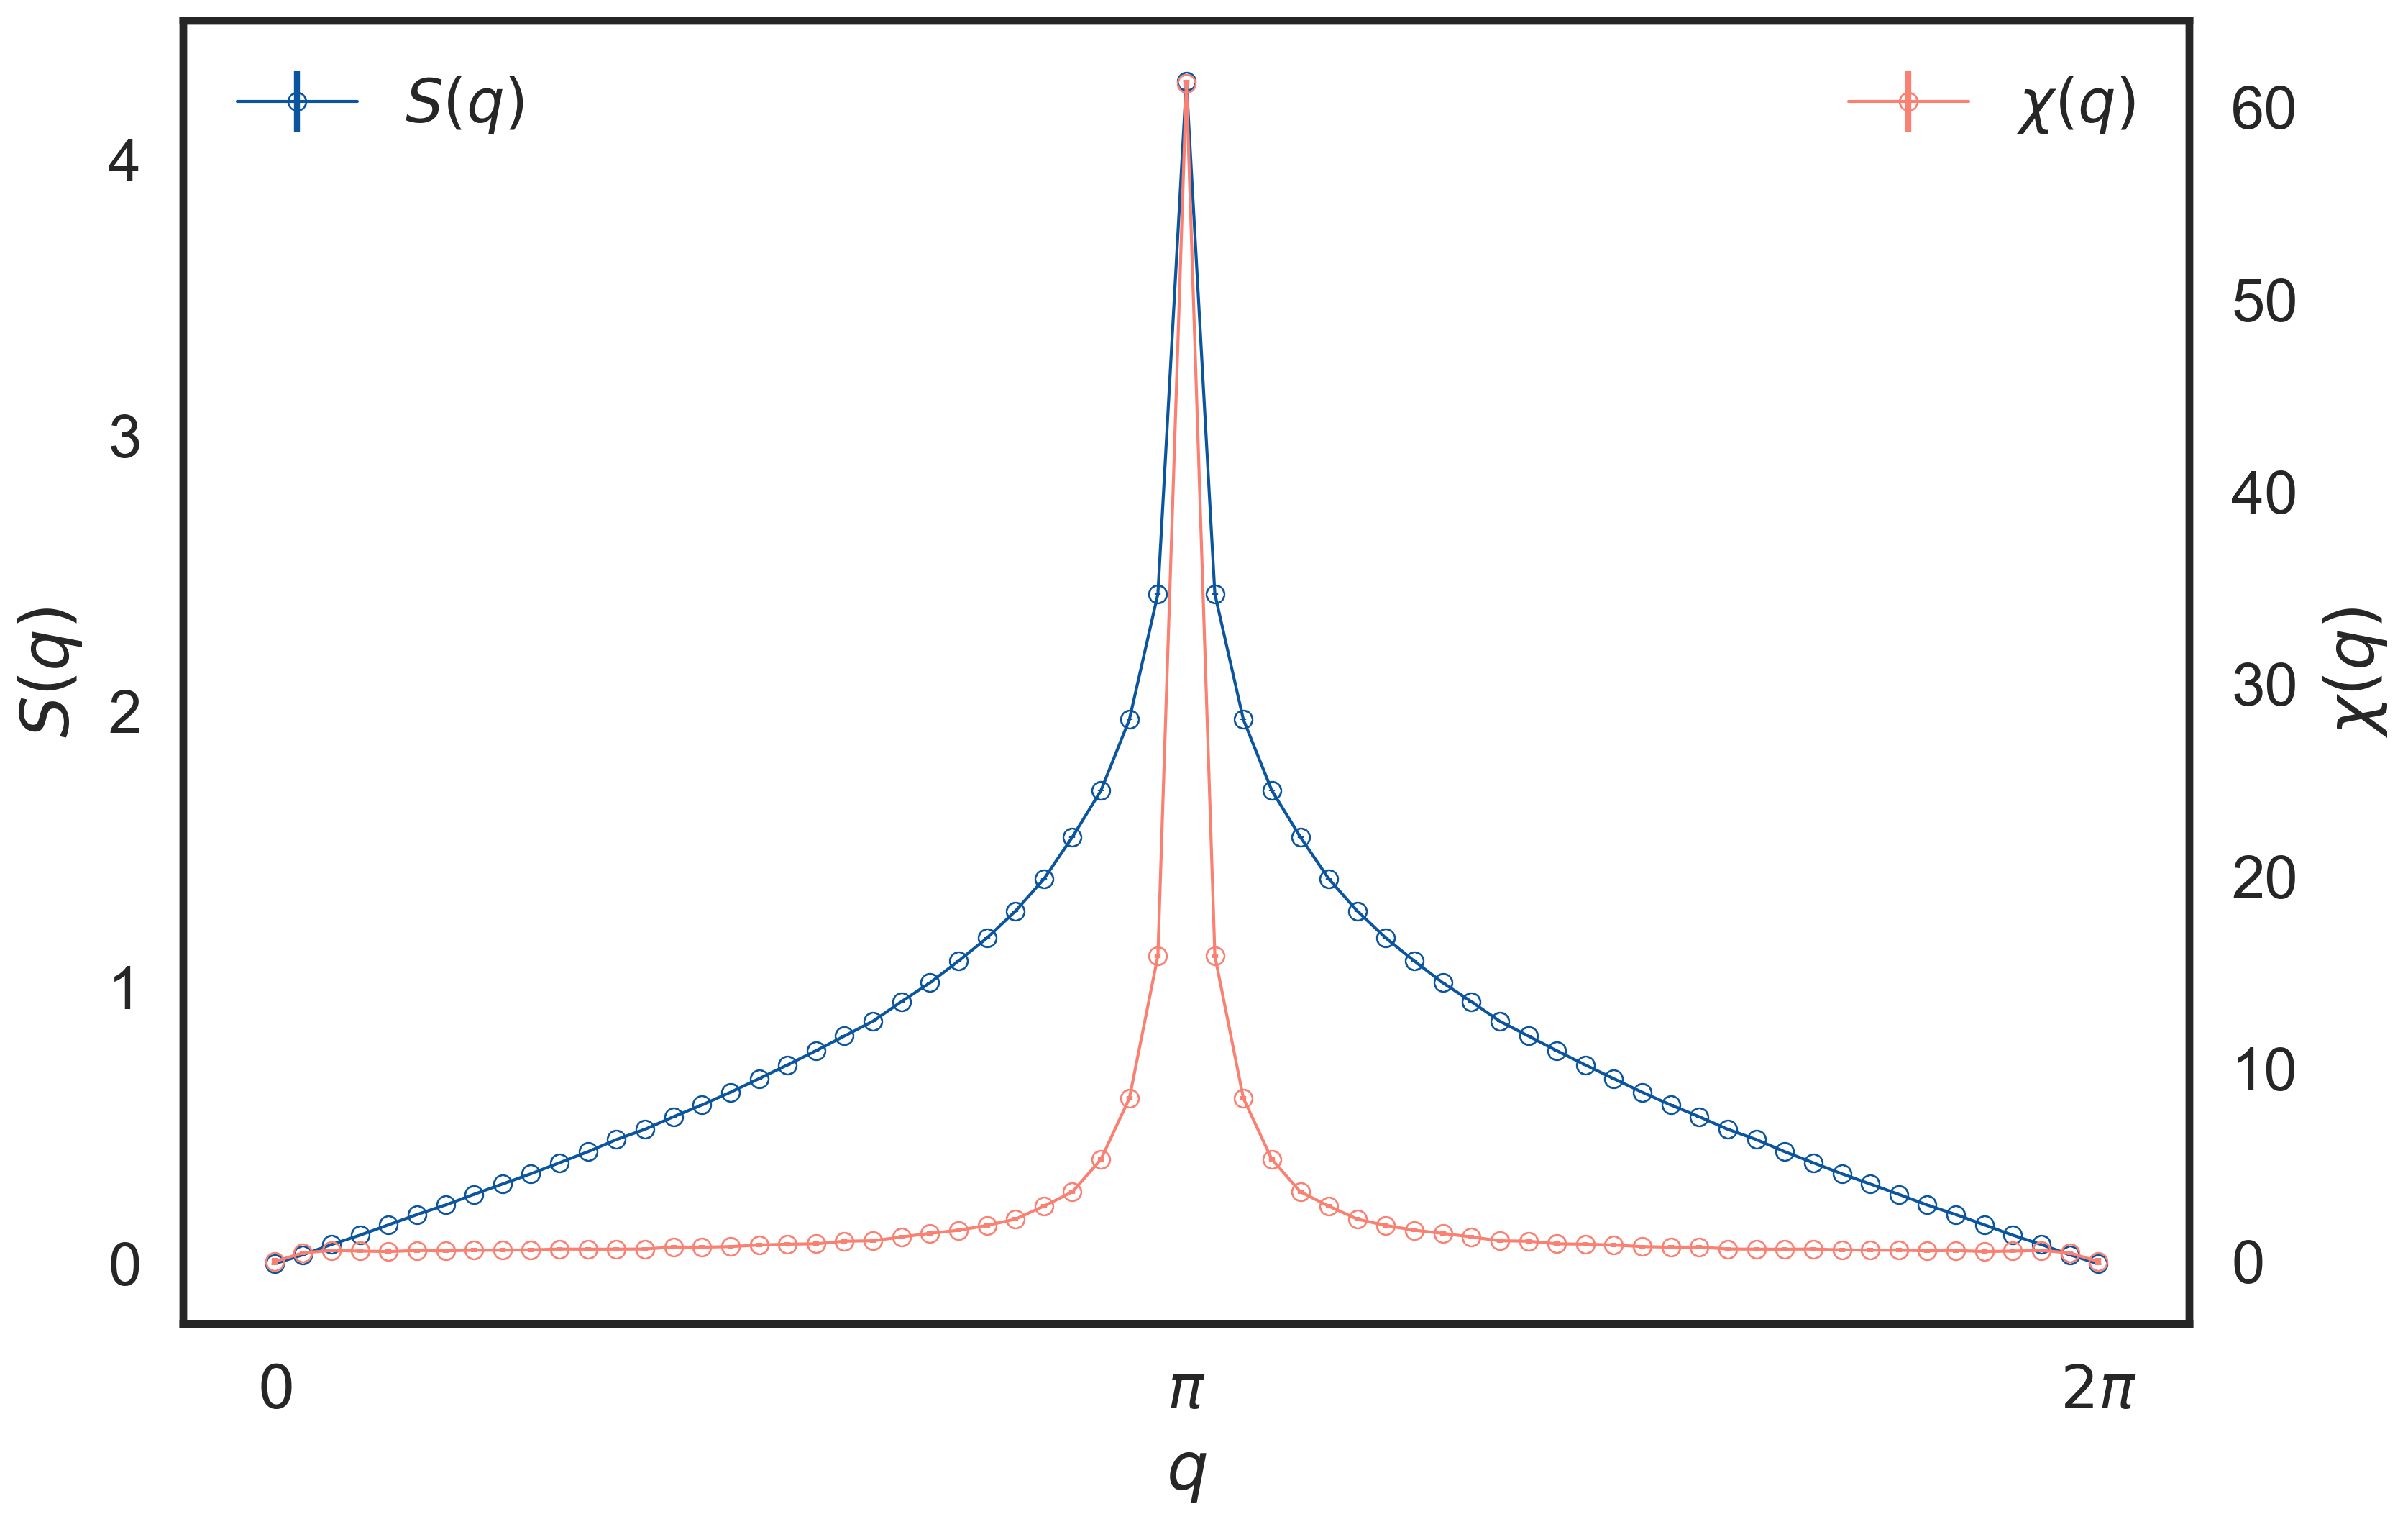
\includegraphics[scale=0.53]{Applications/SandChi.png}
\caption[Spin-spin correlation function, magnetic structure factor, and susceptibility for a 64 site Hubbard chain at $\beta = 25 t$, for $U = 4t$.]{Left: Spin-spin correlation function $\left\langle S^z_i S^z_j \right\rangle$ centered on the middle of the chain.
Right: Magnetic structure factor, and susceptibility (right) for a 64 site Hubbard chain at $\beta = 25 t$, for $U = 4t$, at half filling $\left\langle n \right\rangle = 1$.}
\end{figure}
%According to spin-wave theory, the magnetic susceptiblity can be obtained from the spin-wave dispersion relation $\varepsilon ( k ) \propto k$, and at low temperature, we have
%\begin{equation}
%\chi \propto \int k dk \frac{e^{\beta k}}{(e^{\beta k} -1)^2} \propto T \ln T
%\end{equation}
%
%We find that within statistical uncertainty (which is bigger for $q=0$ for both the structure factor and the susceptibility), our results match this limit at low temperature already at $U = 4t$ (see Fig.(\ref{fig:Schi0})).
%\begin{figure}[H]
%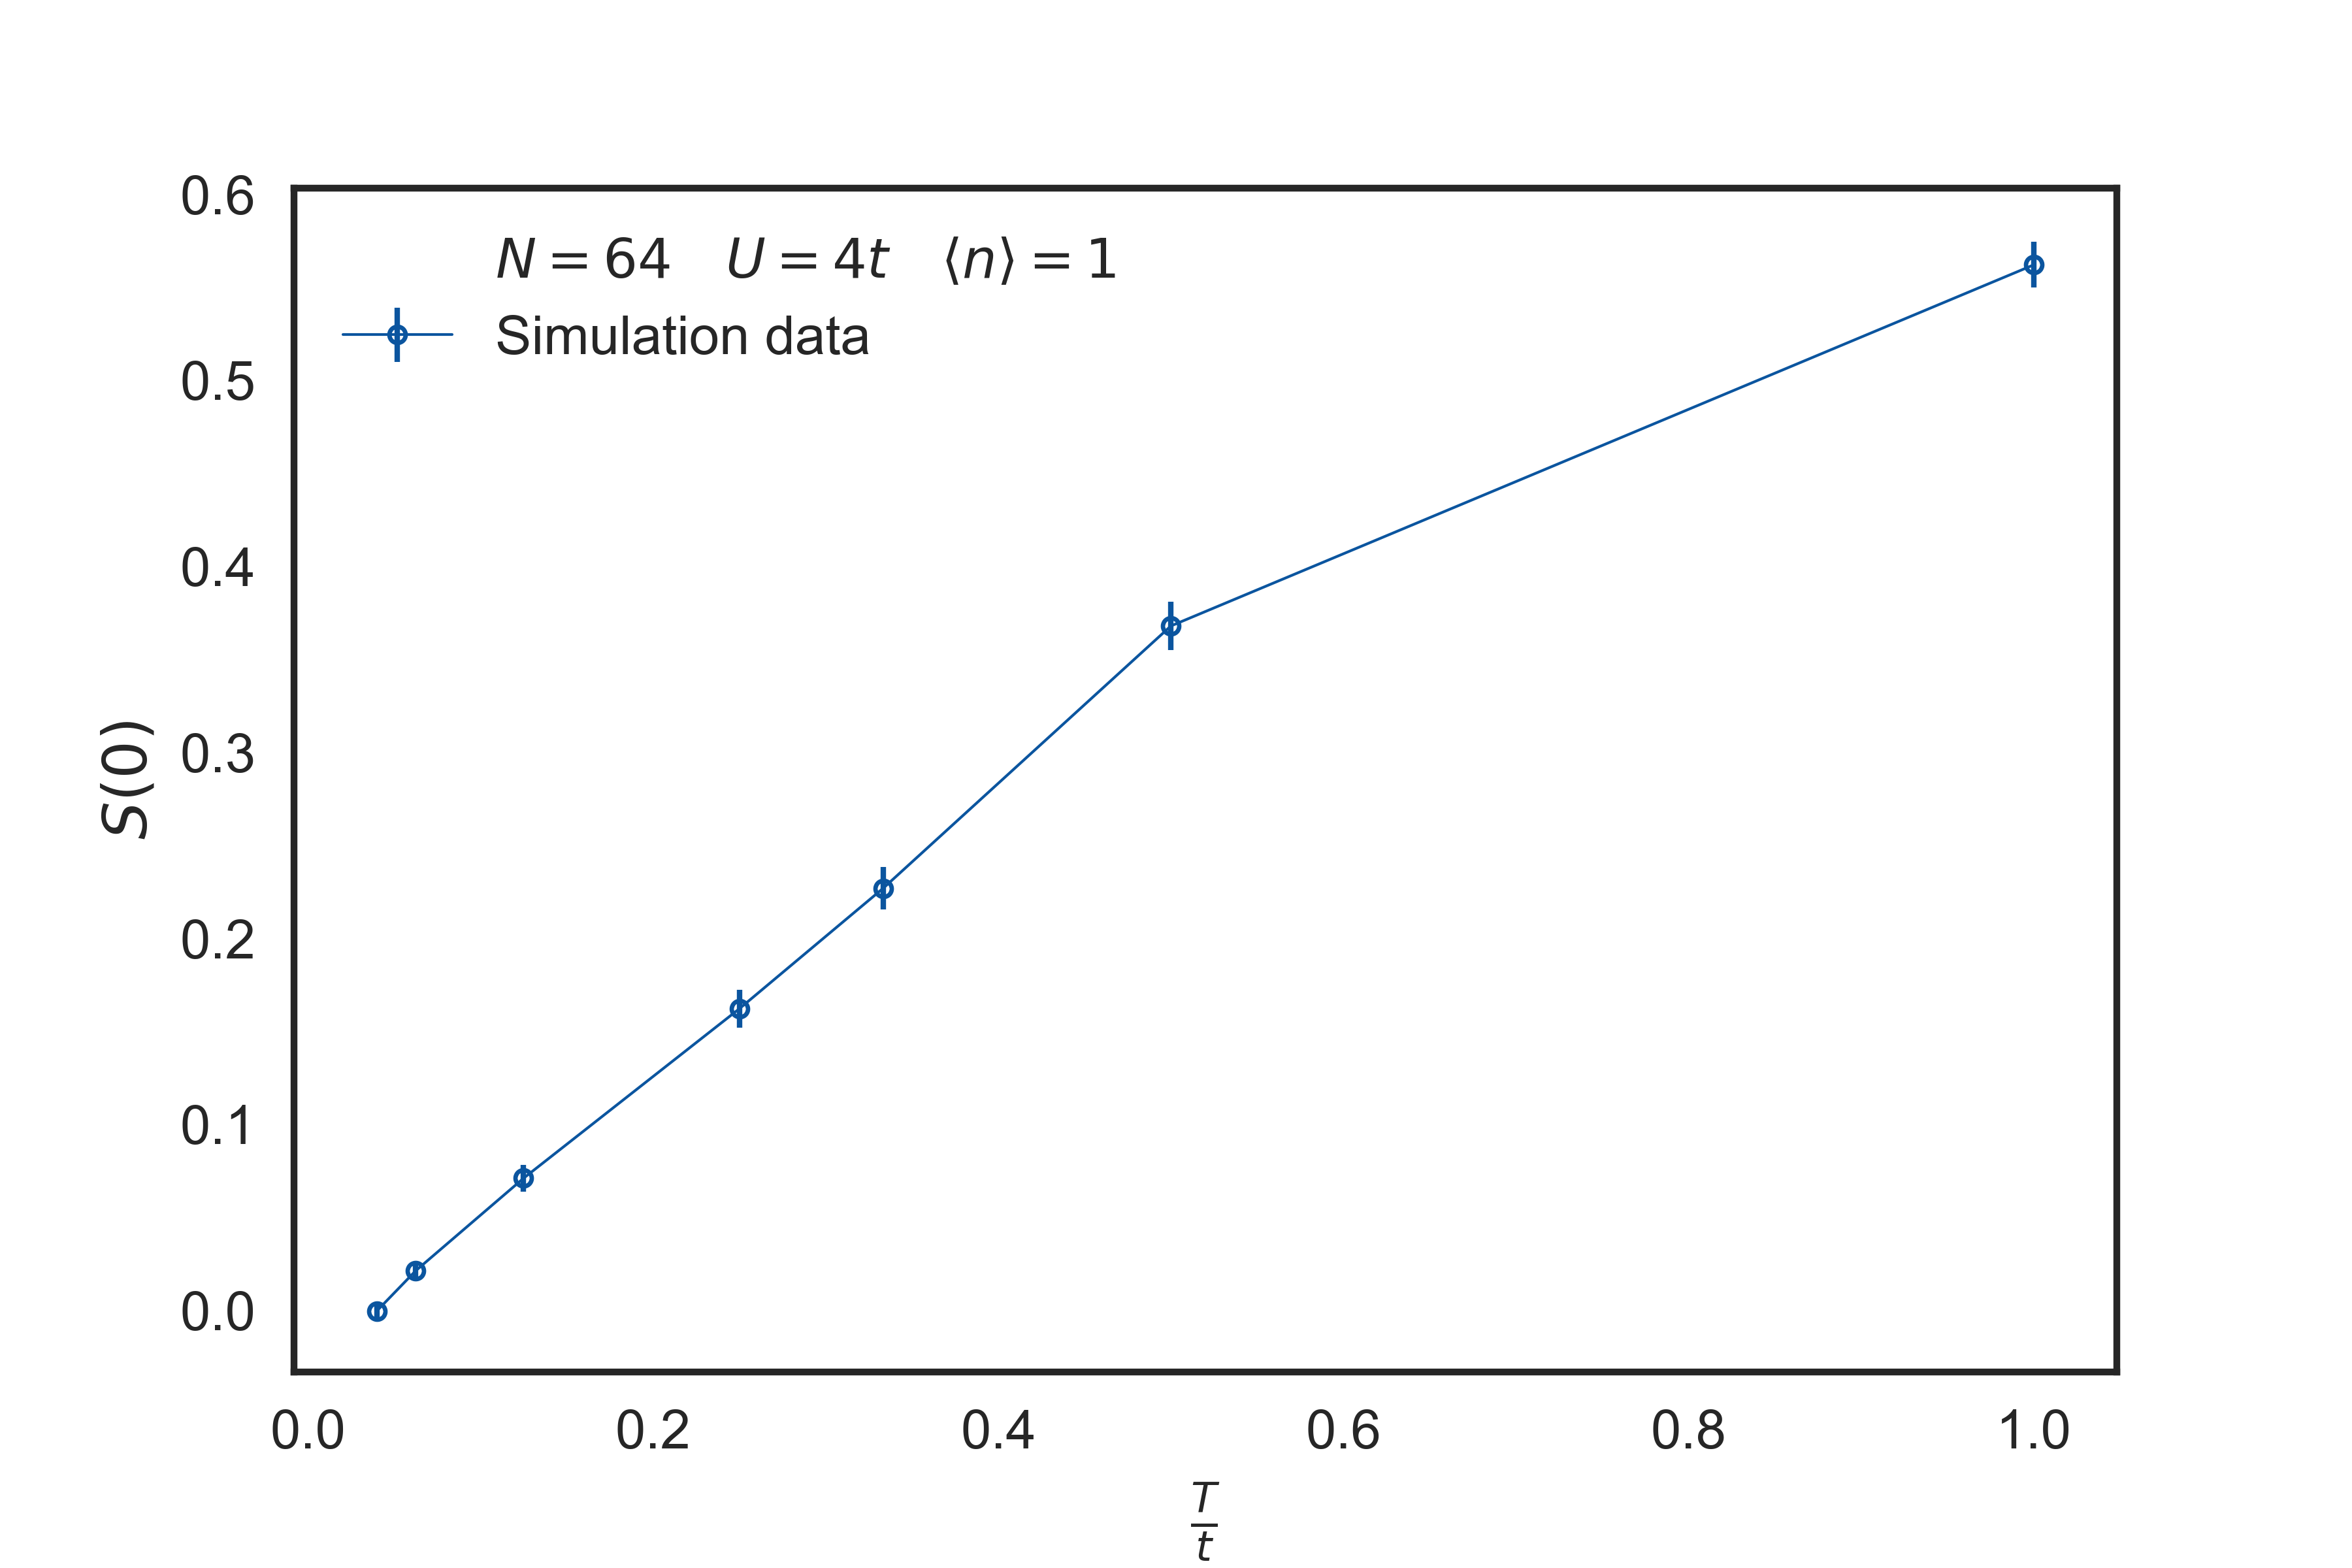
\includegraphics[scale=0.53]{Applications/S0T.png}
%\hspace{-0.5cm}
%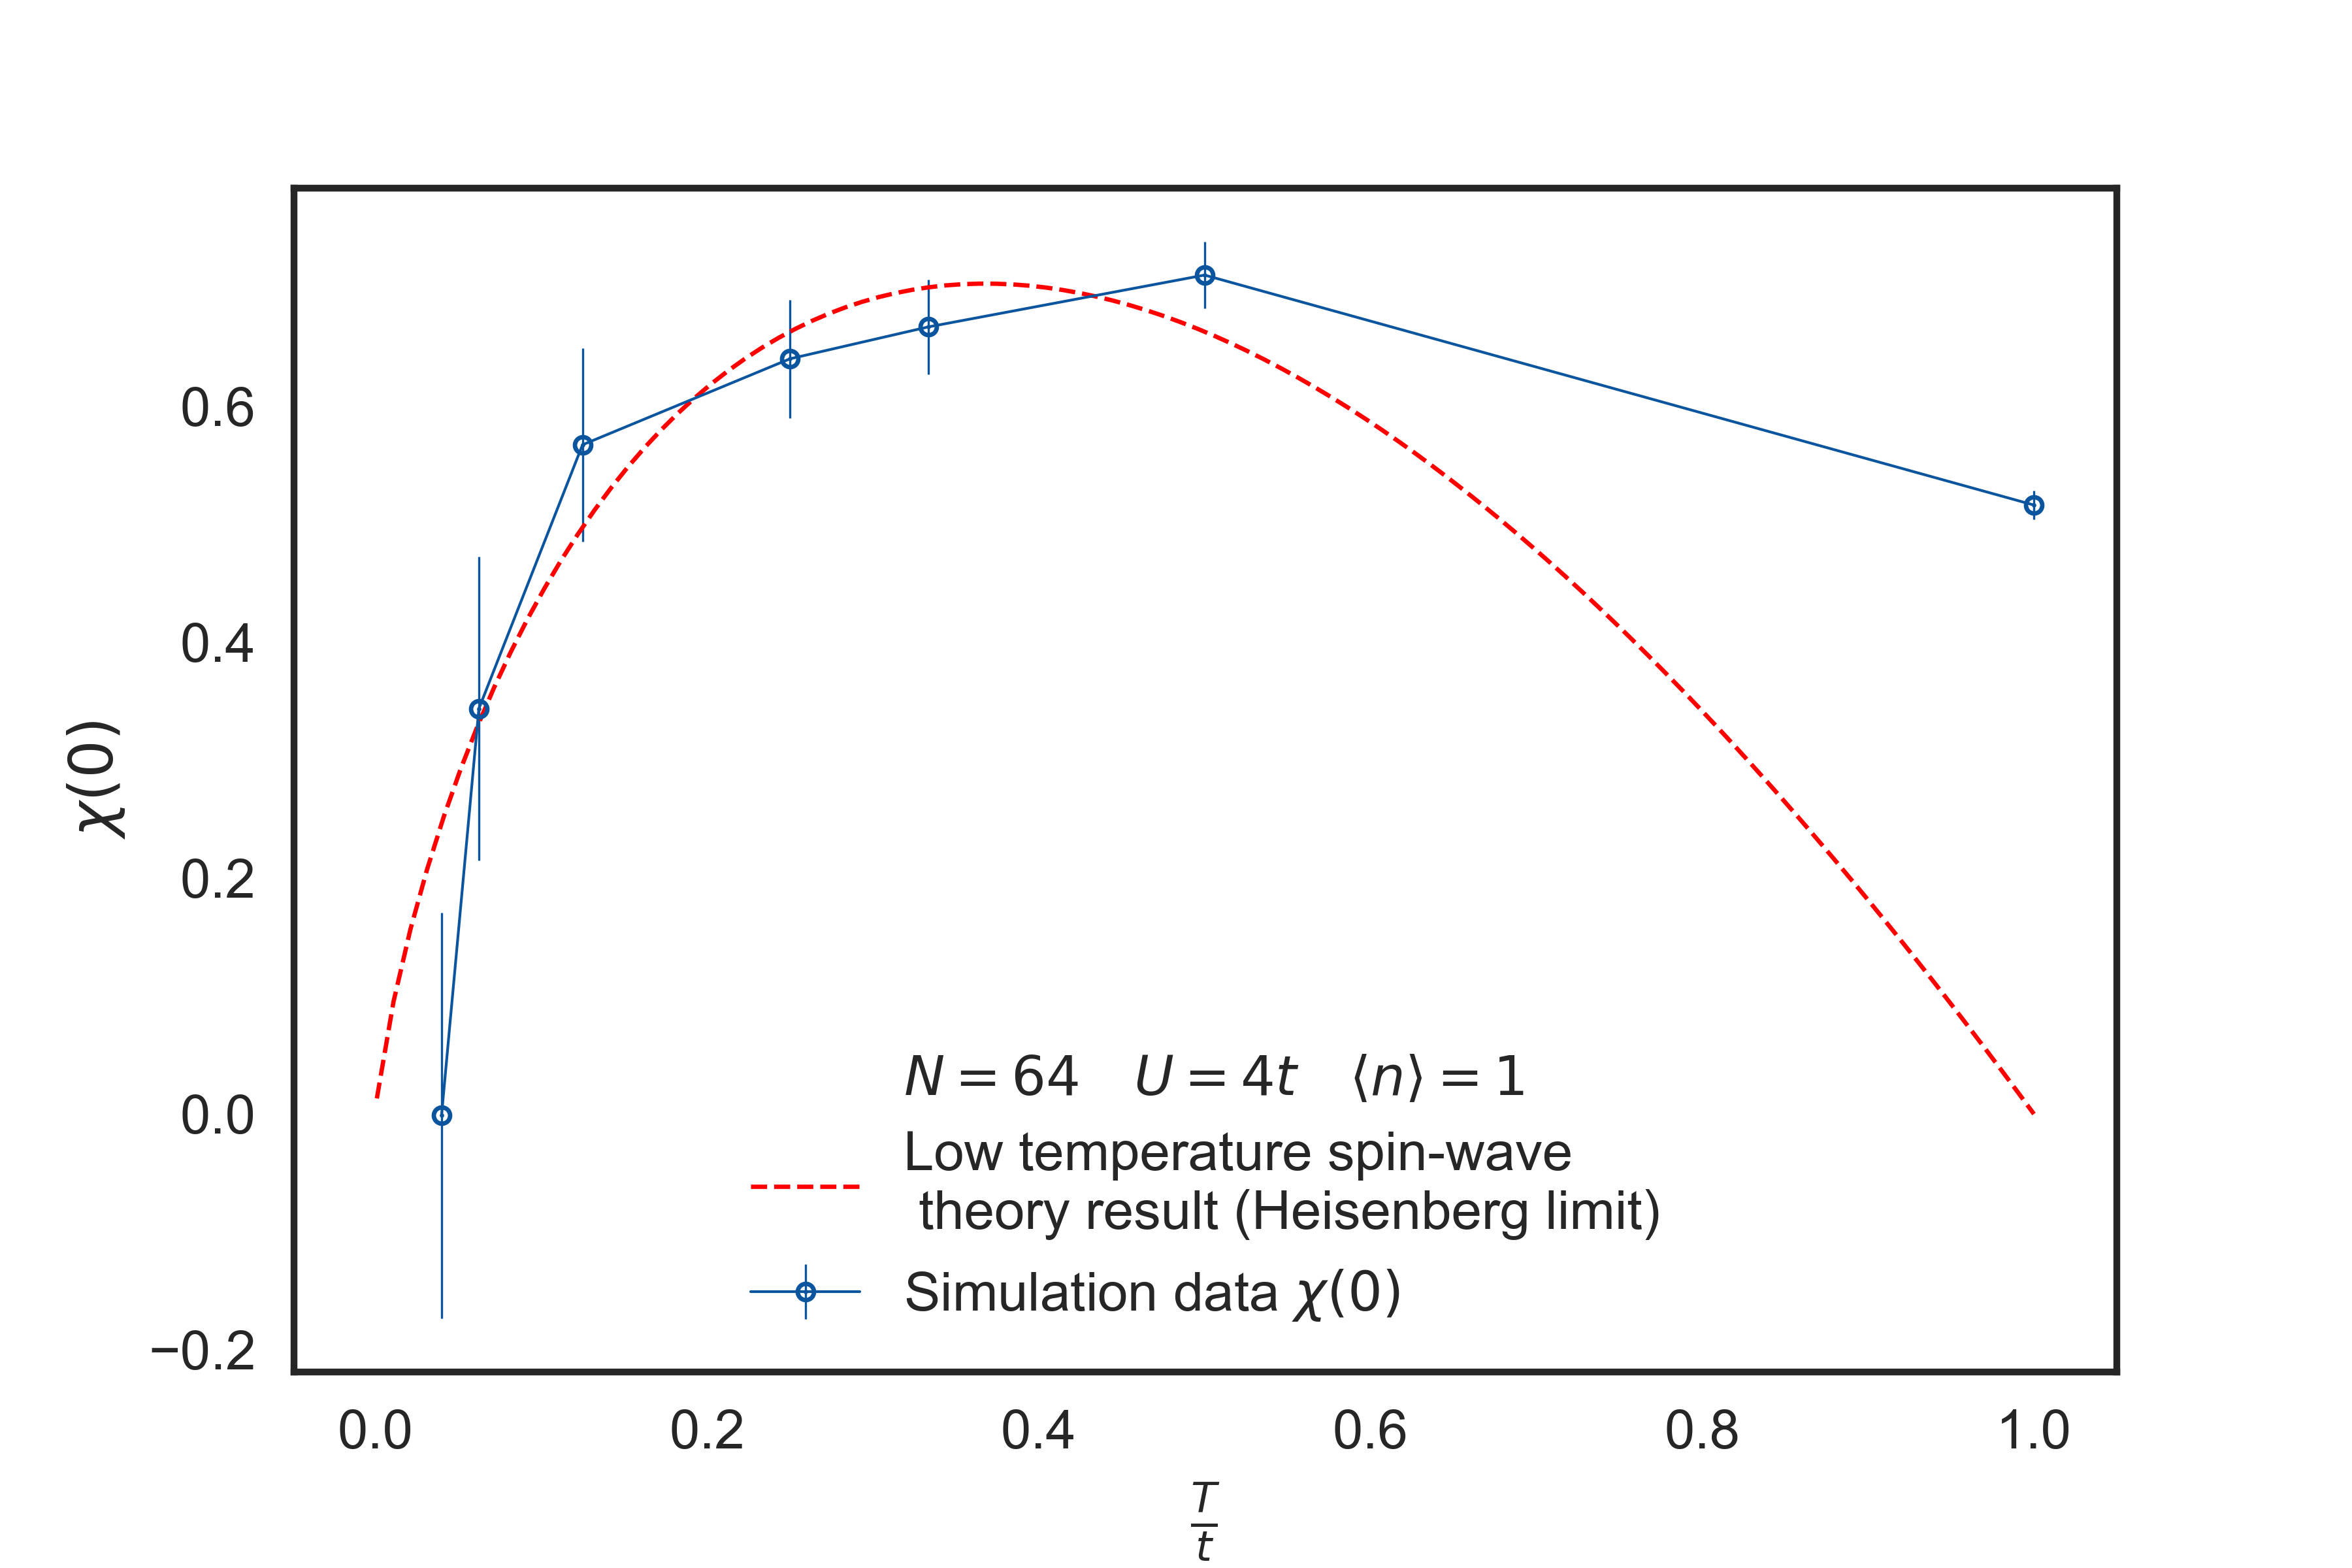
\includegraphics[scale=0.53]{Applications/Sus.png}
%\caption[$q=0$ components of the magnetic structure factor and susceptibility as a function of temperature, indicating that the ground state does not have ferromagnetic ordering.]{By performing simulations for varying temperature and looking at the $q=0$ components of the magnetic structure factor and susceptibility as a function of temperature, we see that the ground state does not have ferromagnetic ordering.
%Furthermore, our result agrees with the low temperature prediction of spin-wave theory for the Heisenberg model, the large $U$ limit of the Hubbard model.\label{fig:Schi0}}
%\end{figure}
In the Heisenberg limit $U \gg t$, the staggered susceptibility $\chi_{\text{st}} \equiv \chi (\pi)$ diverges as $\chi_{\text{st}} ( T ) \propto 1 / (T - T_c) $.
Already at $U = 4 t$, we find exactly this behavior with a critical temperature $T_c$ very close to zero.
\begin{figure}[H]\label{fig:SchiPi}
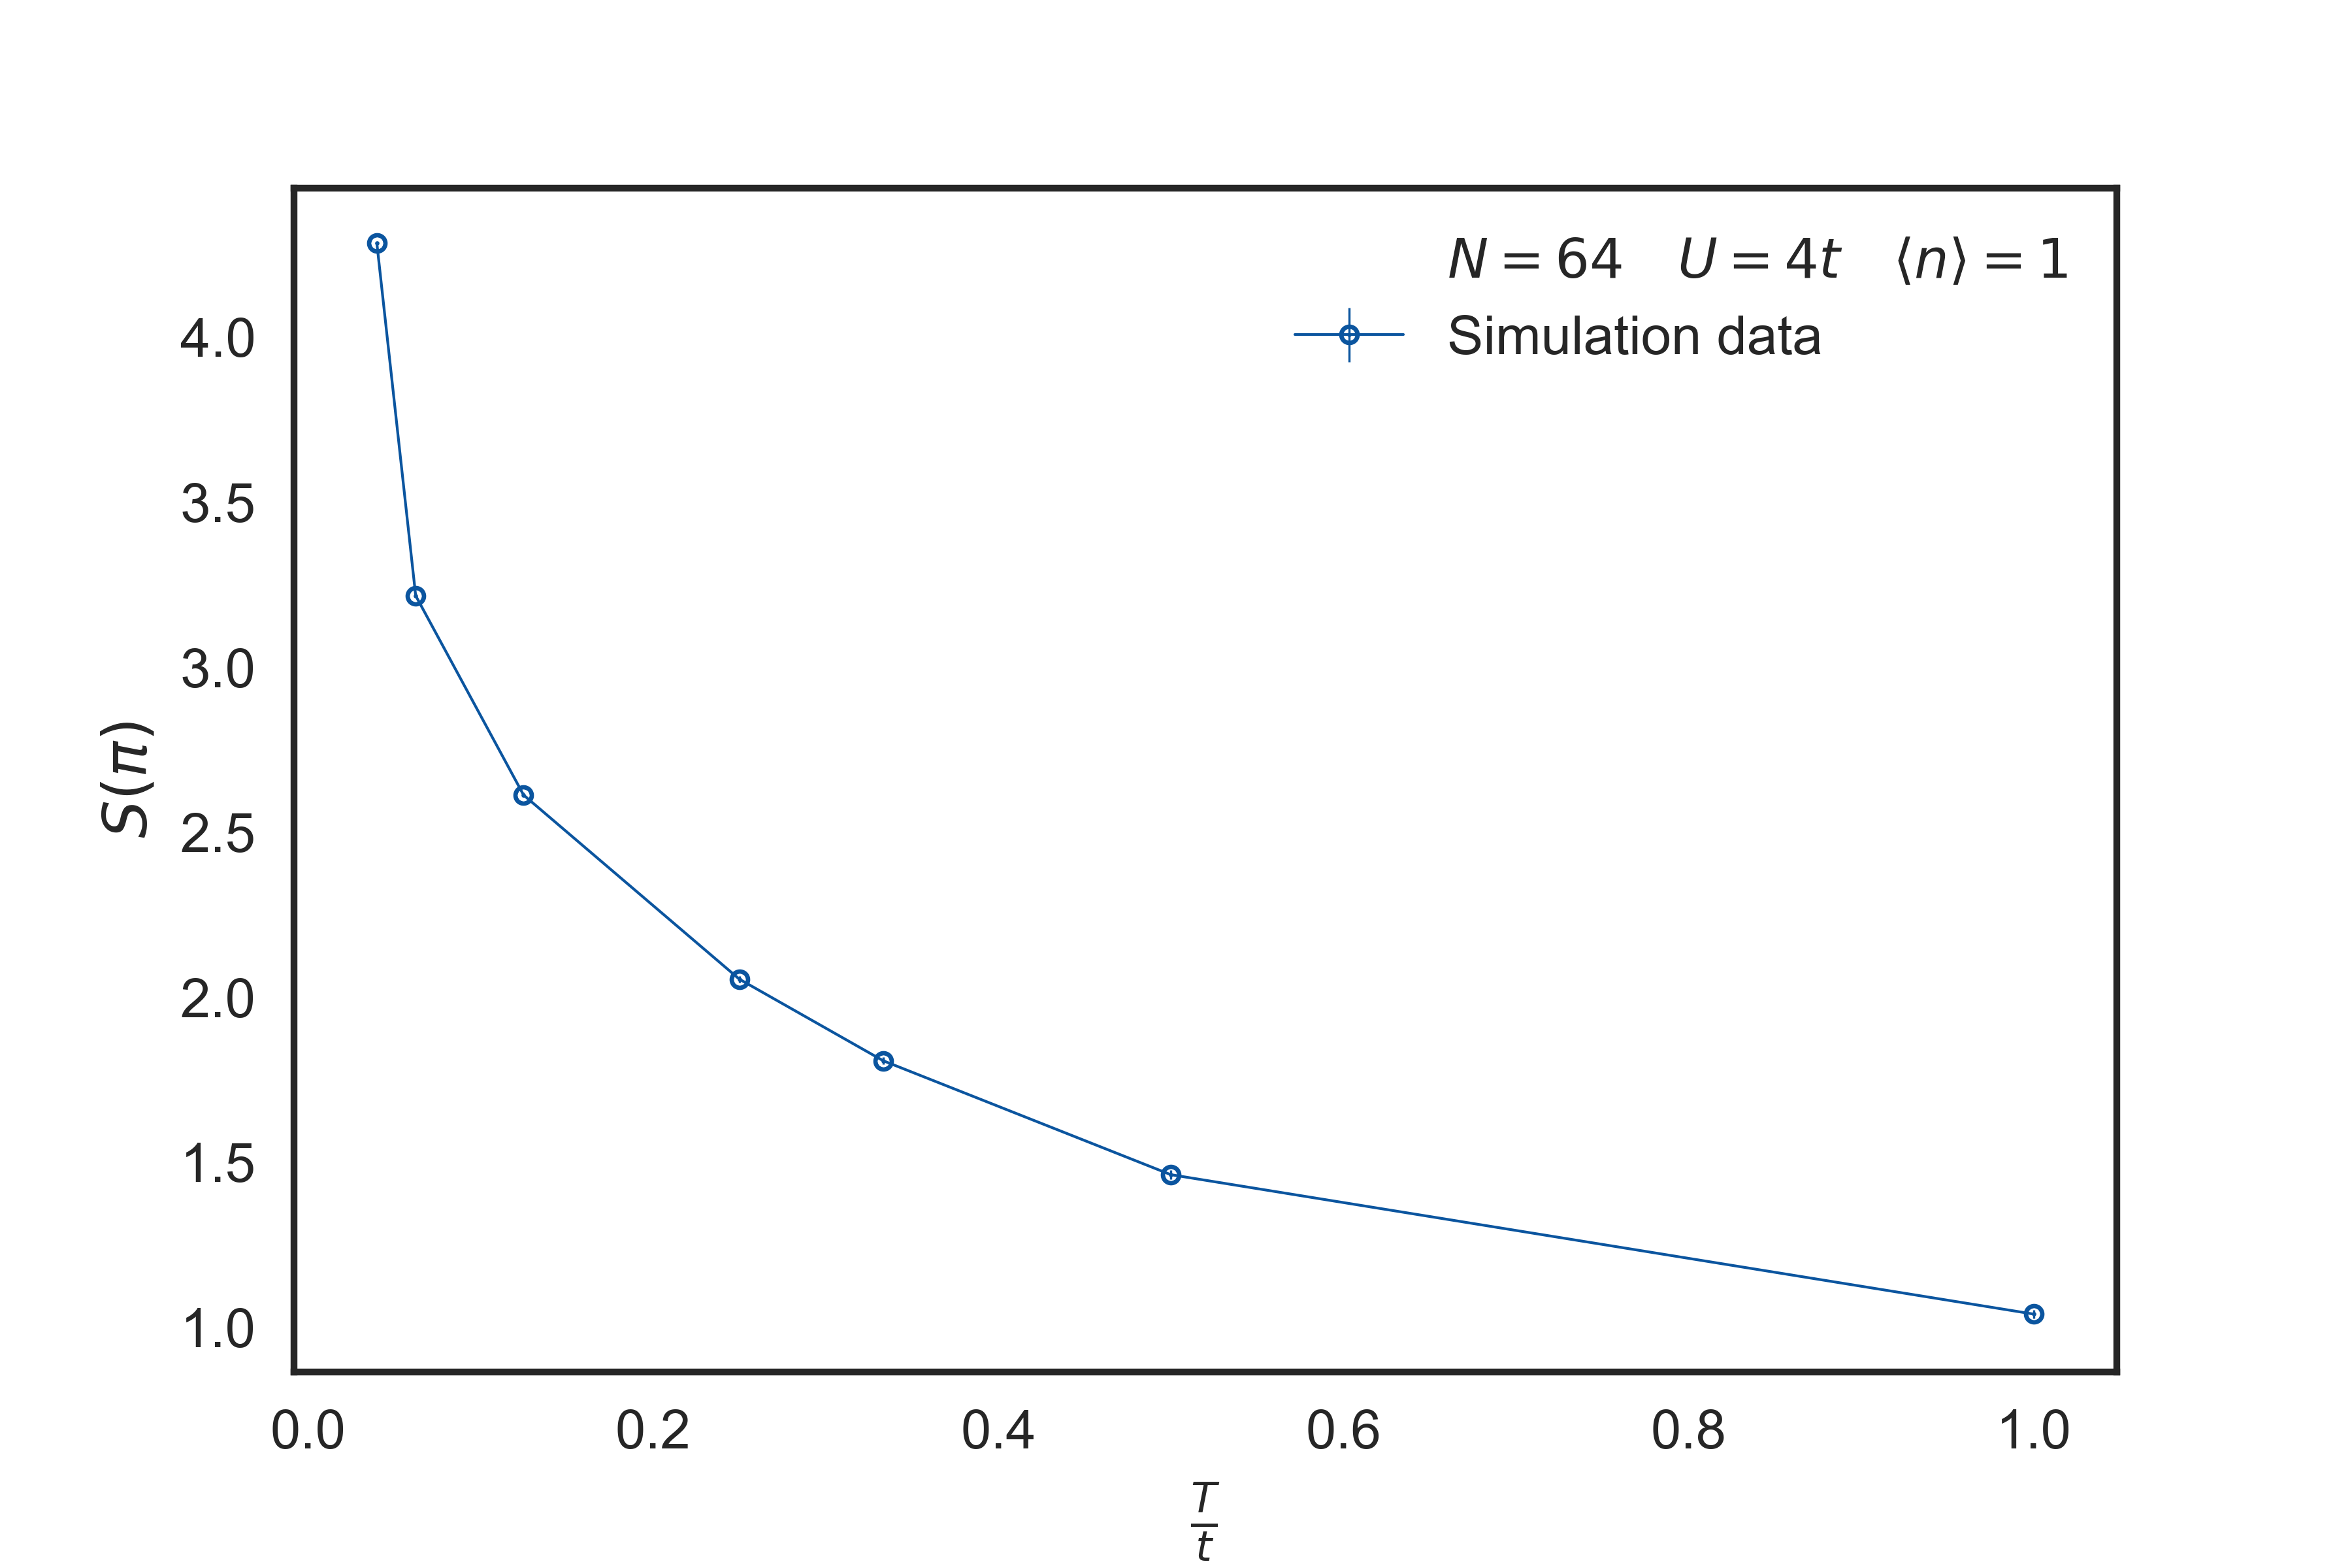
\includegraphics[scale=0.53]{Applications/SqT.png}
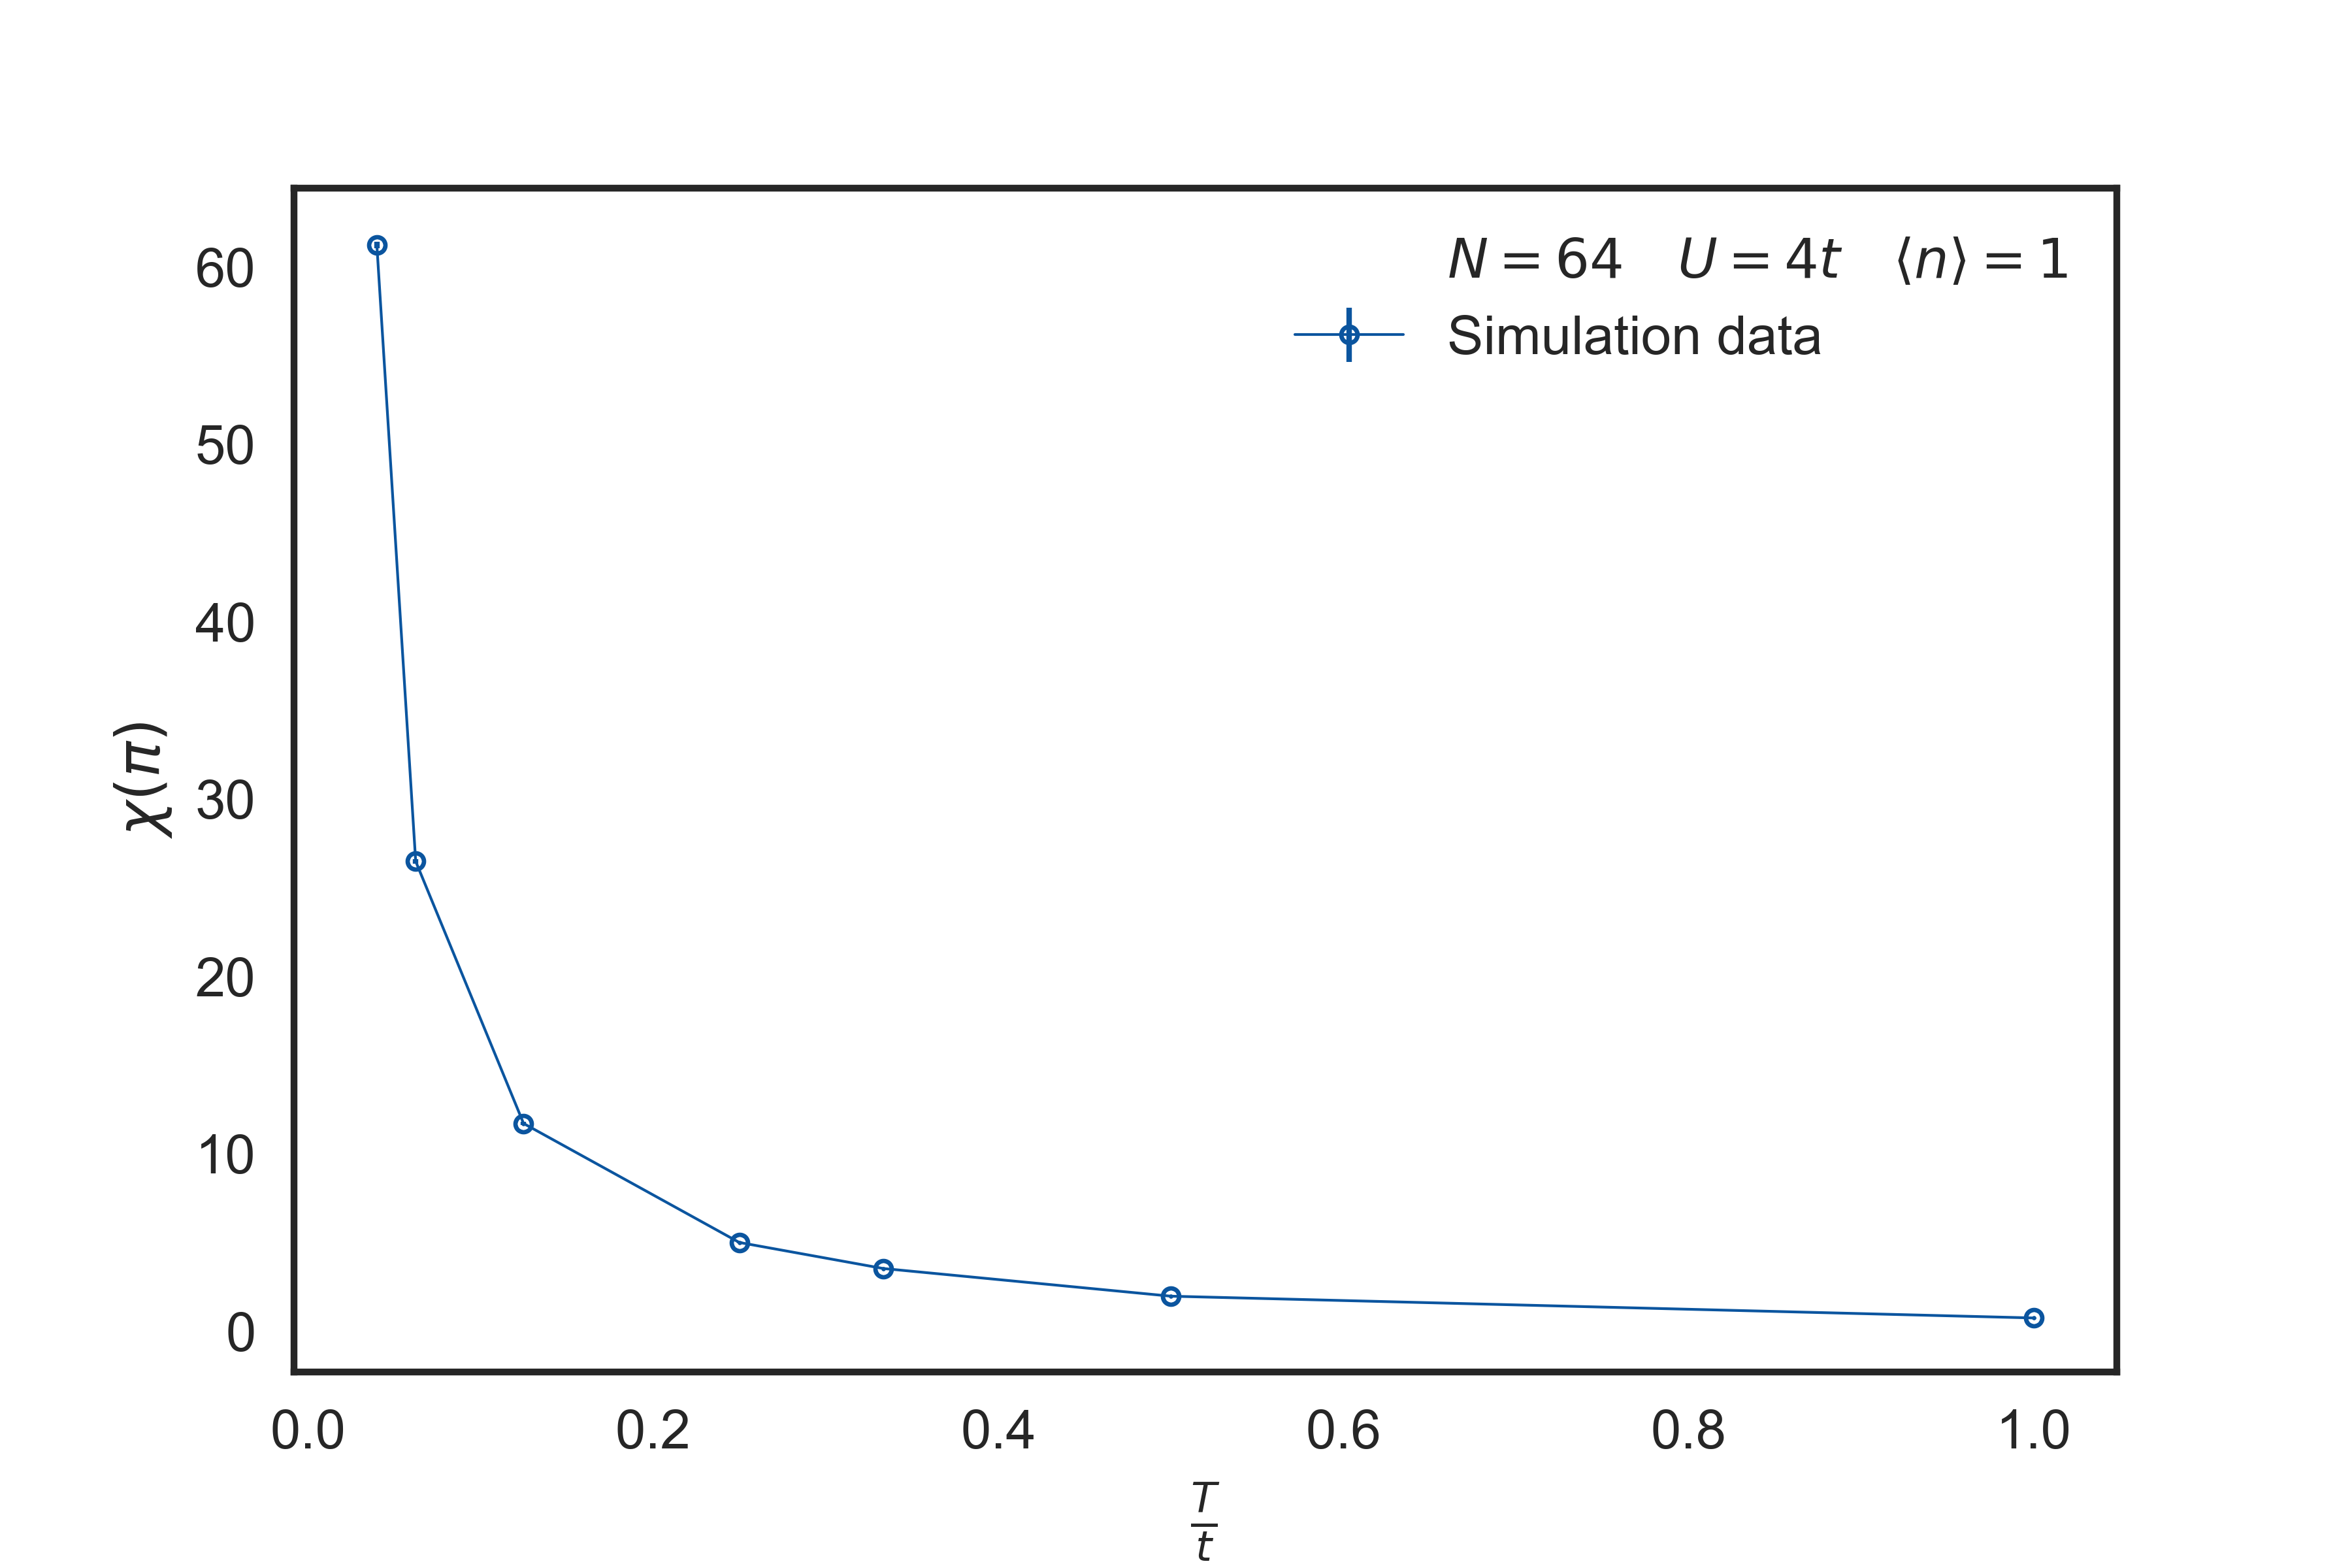
\includegraphics[scale=0.53]{Applications/stSus.png}
\caption[The magnetic structure factor and the  susceptibility have a peak at $q = \pi$ that increases as $T\rightarrow 0$, indicating \emph{antiferromagnetic ordering}.
 Divergence of the staggered susceptibility near $T_c = 0$, signaling the transition to the antiferromagnetic ground state.]{The magnetic structure factor and the susceptibility have a peak at $q = \pi$ that increases as $T\rightarrow 0$, indicating antiferromagnetic ordering.
The staggered susceptibility diverges near $T_c = 0$, signaling the transition to the antiferromagnetic ground state.}
\end{figure}

We ran \texttt{QUEST} for the same 64-site chain we simulated with our code, using $\beta = 25 t$, taking a half filled chain ($\left\langle n \right\rangle = 1$), and setting $U = 4t$.
We found a remarkable agreement between the measurements obtained using our code and using \texttt{QUEST}, namely in the magnetic structure factor, which we show in Fig.(\ref{fig:quest_time}).
Then, we took a small $2$-site system to compare the run time and verify the $\mathcal{O}(L)$ scaling of the determinant \ac{QMC} algorithm.
We noticed that \texttt{QUEST}'s algorithm suffers from large overhead time if the required precision via the Trotter error $\Delta \tau$, or the inverse temperature $\beta$ are large. 
This is due to the pre-conditioning needed to stabilize the products of the larger $L N \times L N$ matrices that are used in their algorithm (ours uses $N \times N$).

The results for the $2$-site system can be compared with the results obtained using exact diagonalization, a method which can only be used for small lattice sizes, and which we outlined in chapter \ref{cap:hubbard}.
We kept all the parameters, changing only the system size, and verified that our results agree with a similar study carried out in \cite{hirsch_discrete_1983}, confirming the validity of our implementation.

\begin{figure}[H]
\hspace{0.1cm}
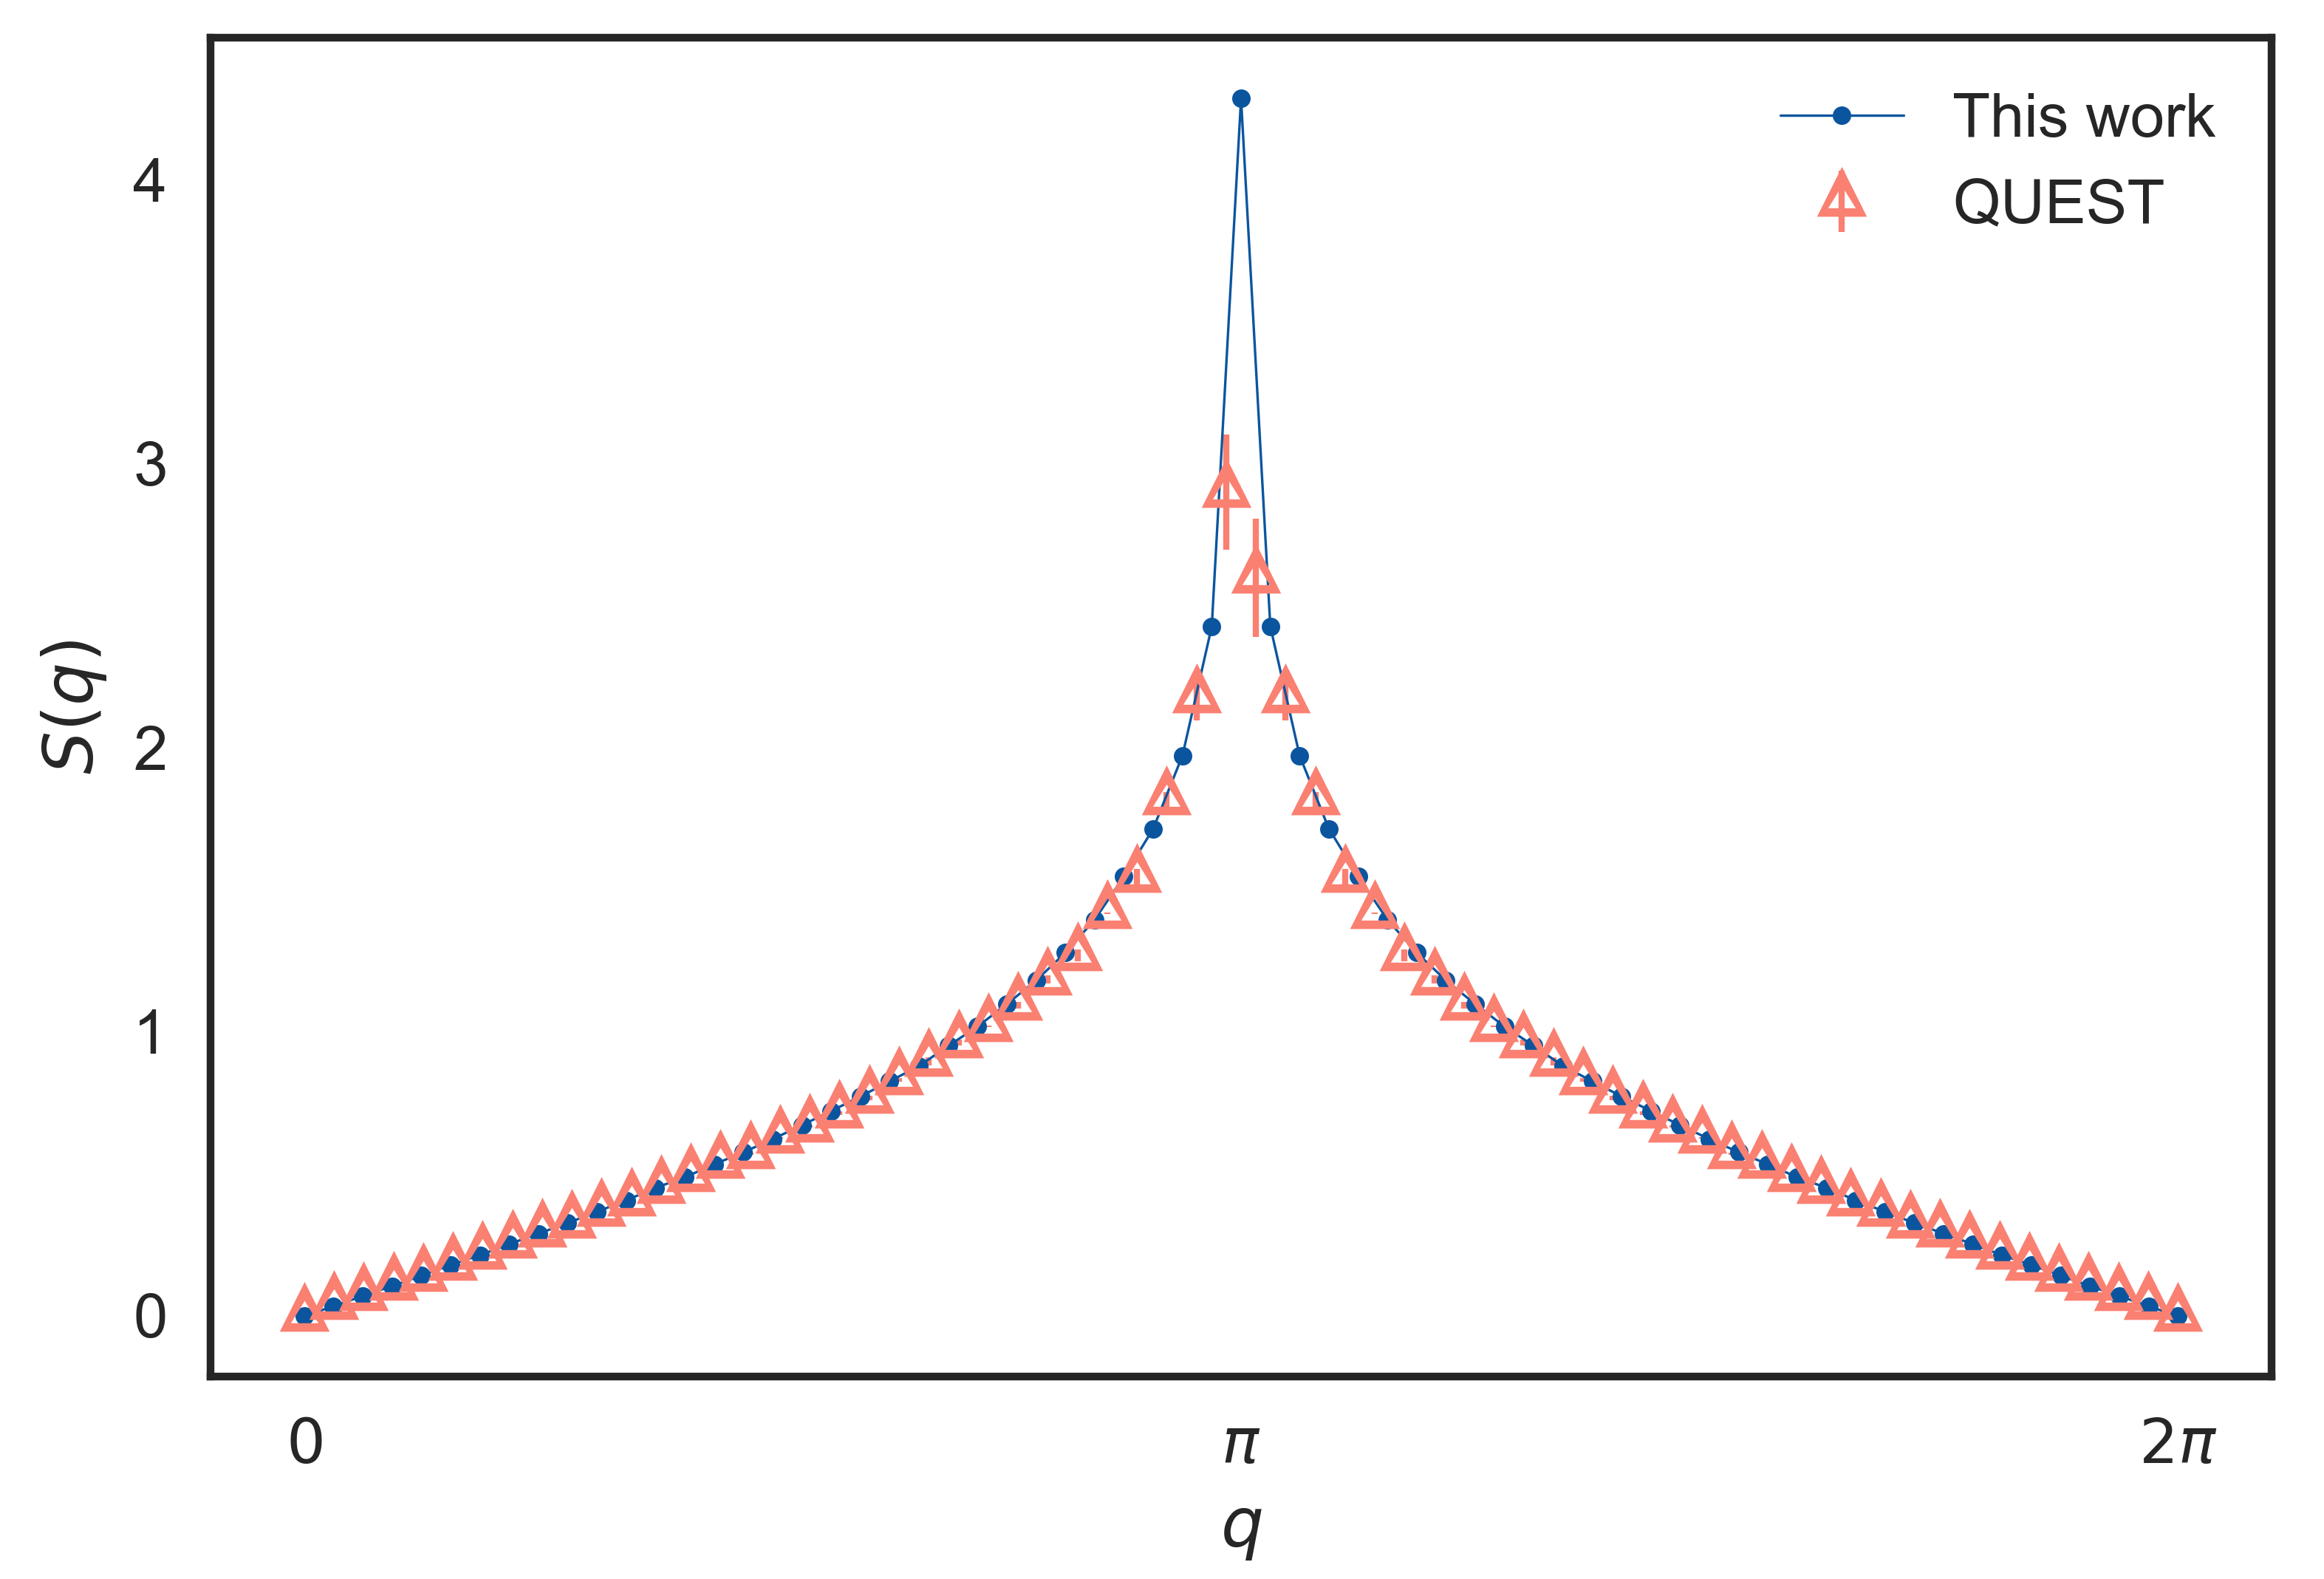
\includegraphics[scale=0.53]{Applications/s_compare.png}
\hspace{0.5cm}
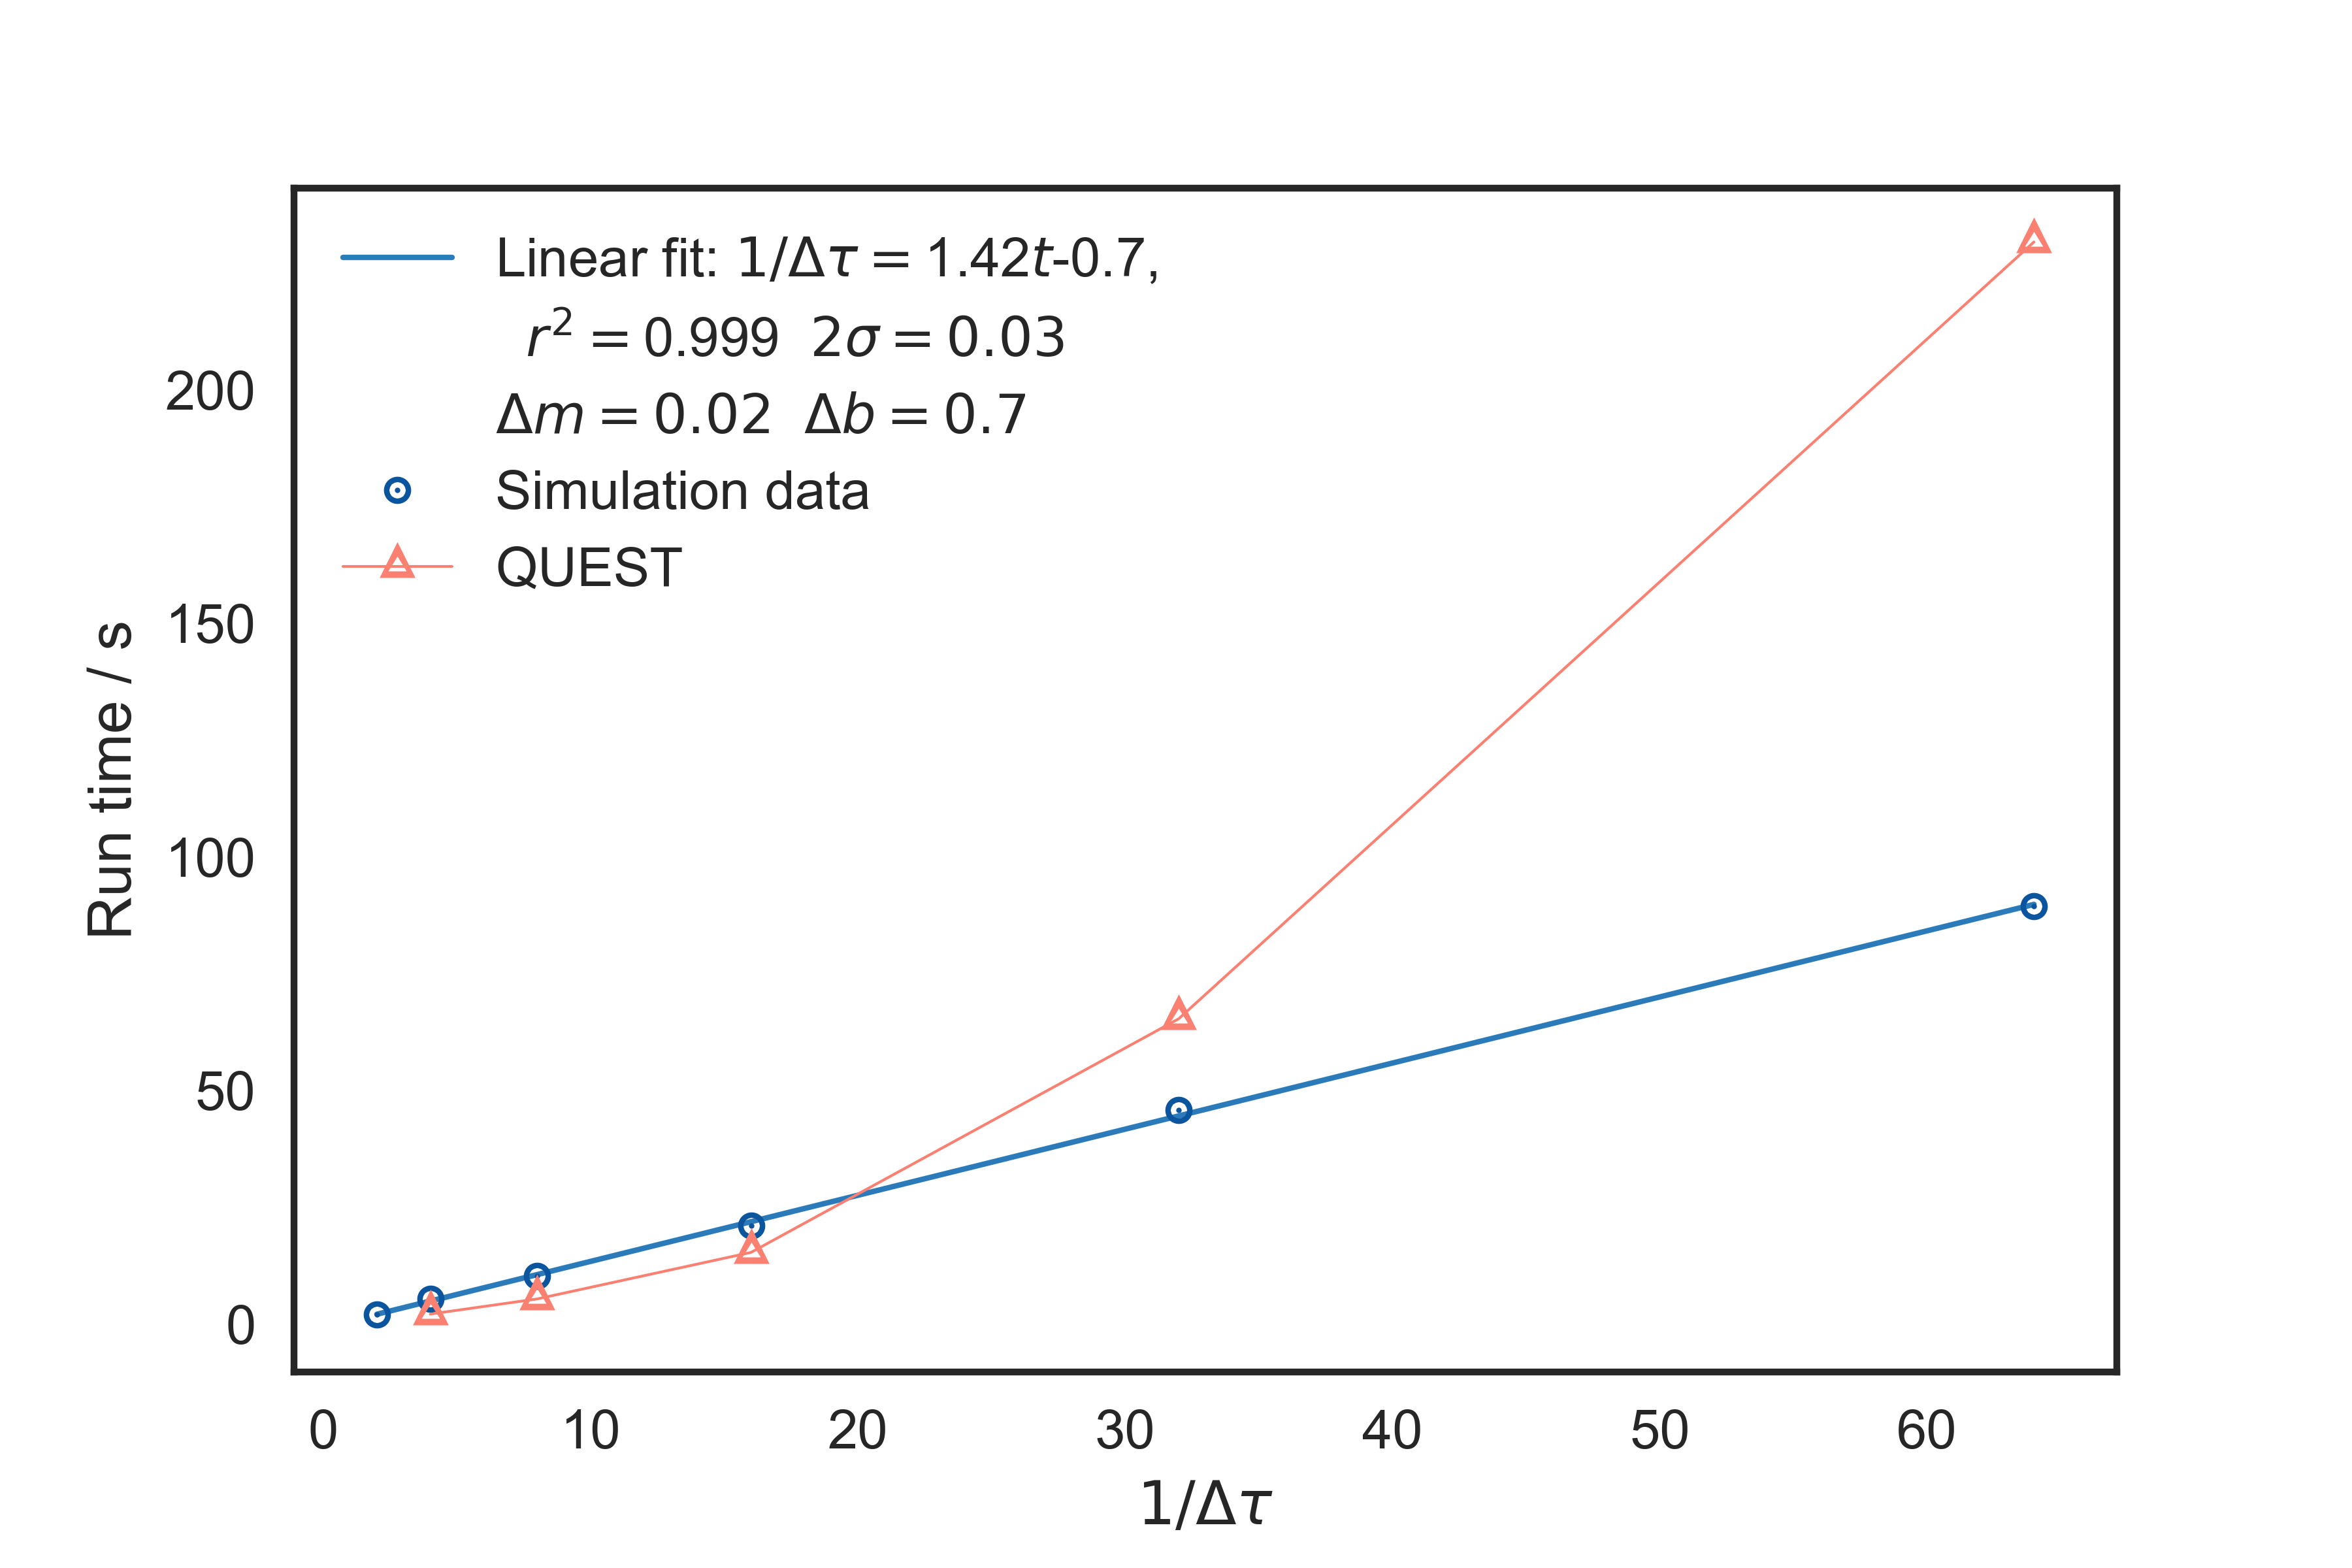
\includegraphics[scale=0.53]{Applications/runtime2sites.png}
\caption[Comparison of the magnetic structure factor with that obtained using \texttt{QUEST}. Run time comparison.]{Left: Comparison of the magnetic structure factor with that obtained using \texttt{QUEST}.
The used parameters are referred in the body of the text.
Right: The run time using our code increases linearly with $L$, as expected.
The \texttt{QUEST} algorithm initially scales linearly, but then becomes much slower due to the large overhead time associated with pre-conditioning the comparably much larger matrices they use if $L$ is very big.\label{fig:quest_time}}
\end{figure}
\begin{figure}[H]\label{fig:hirsch1982}
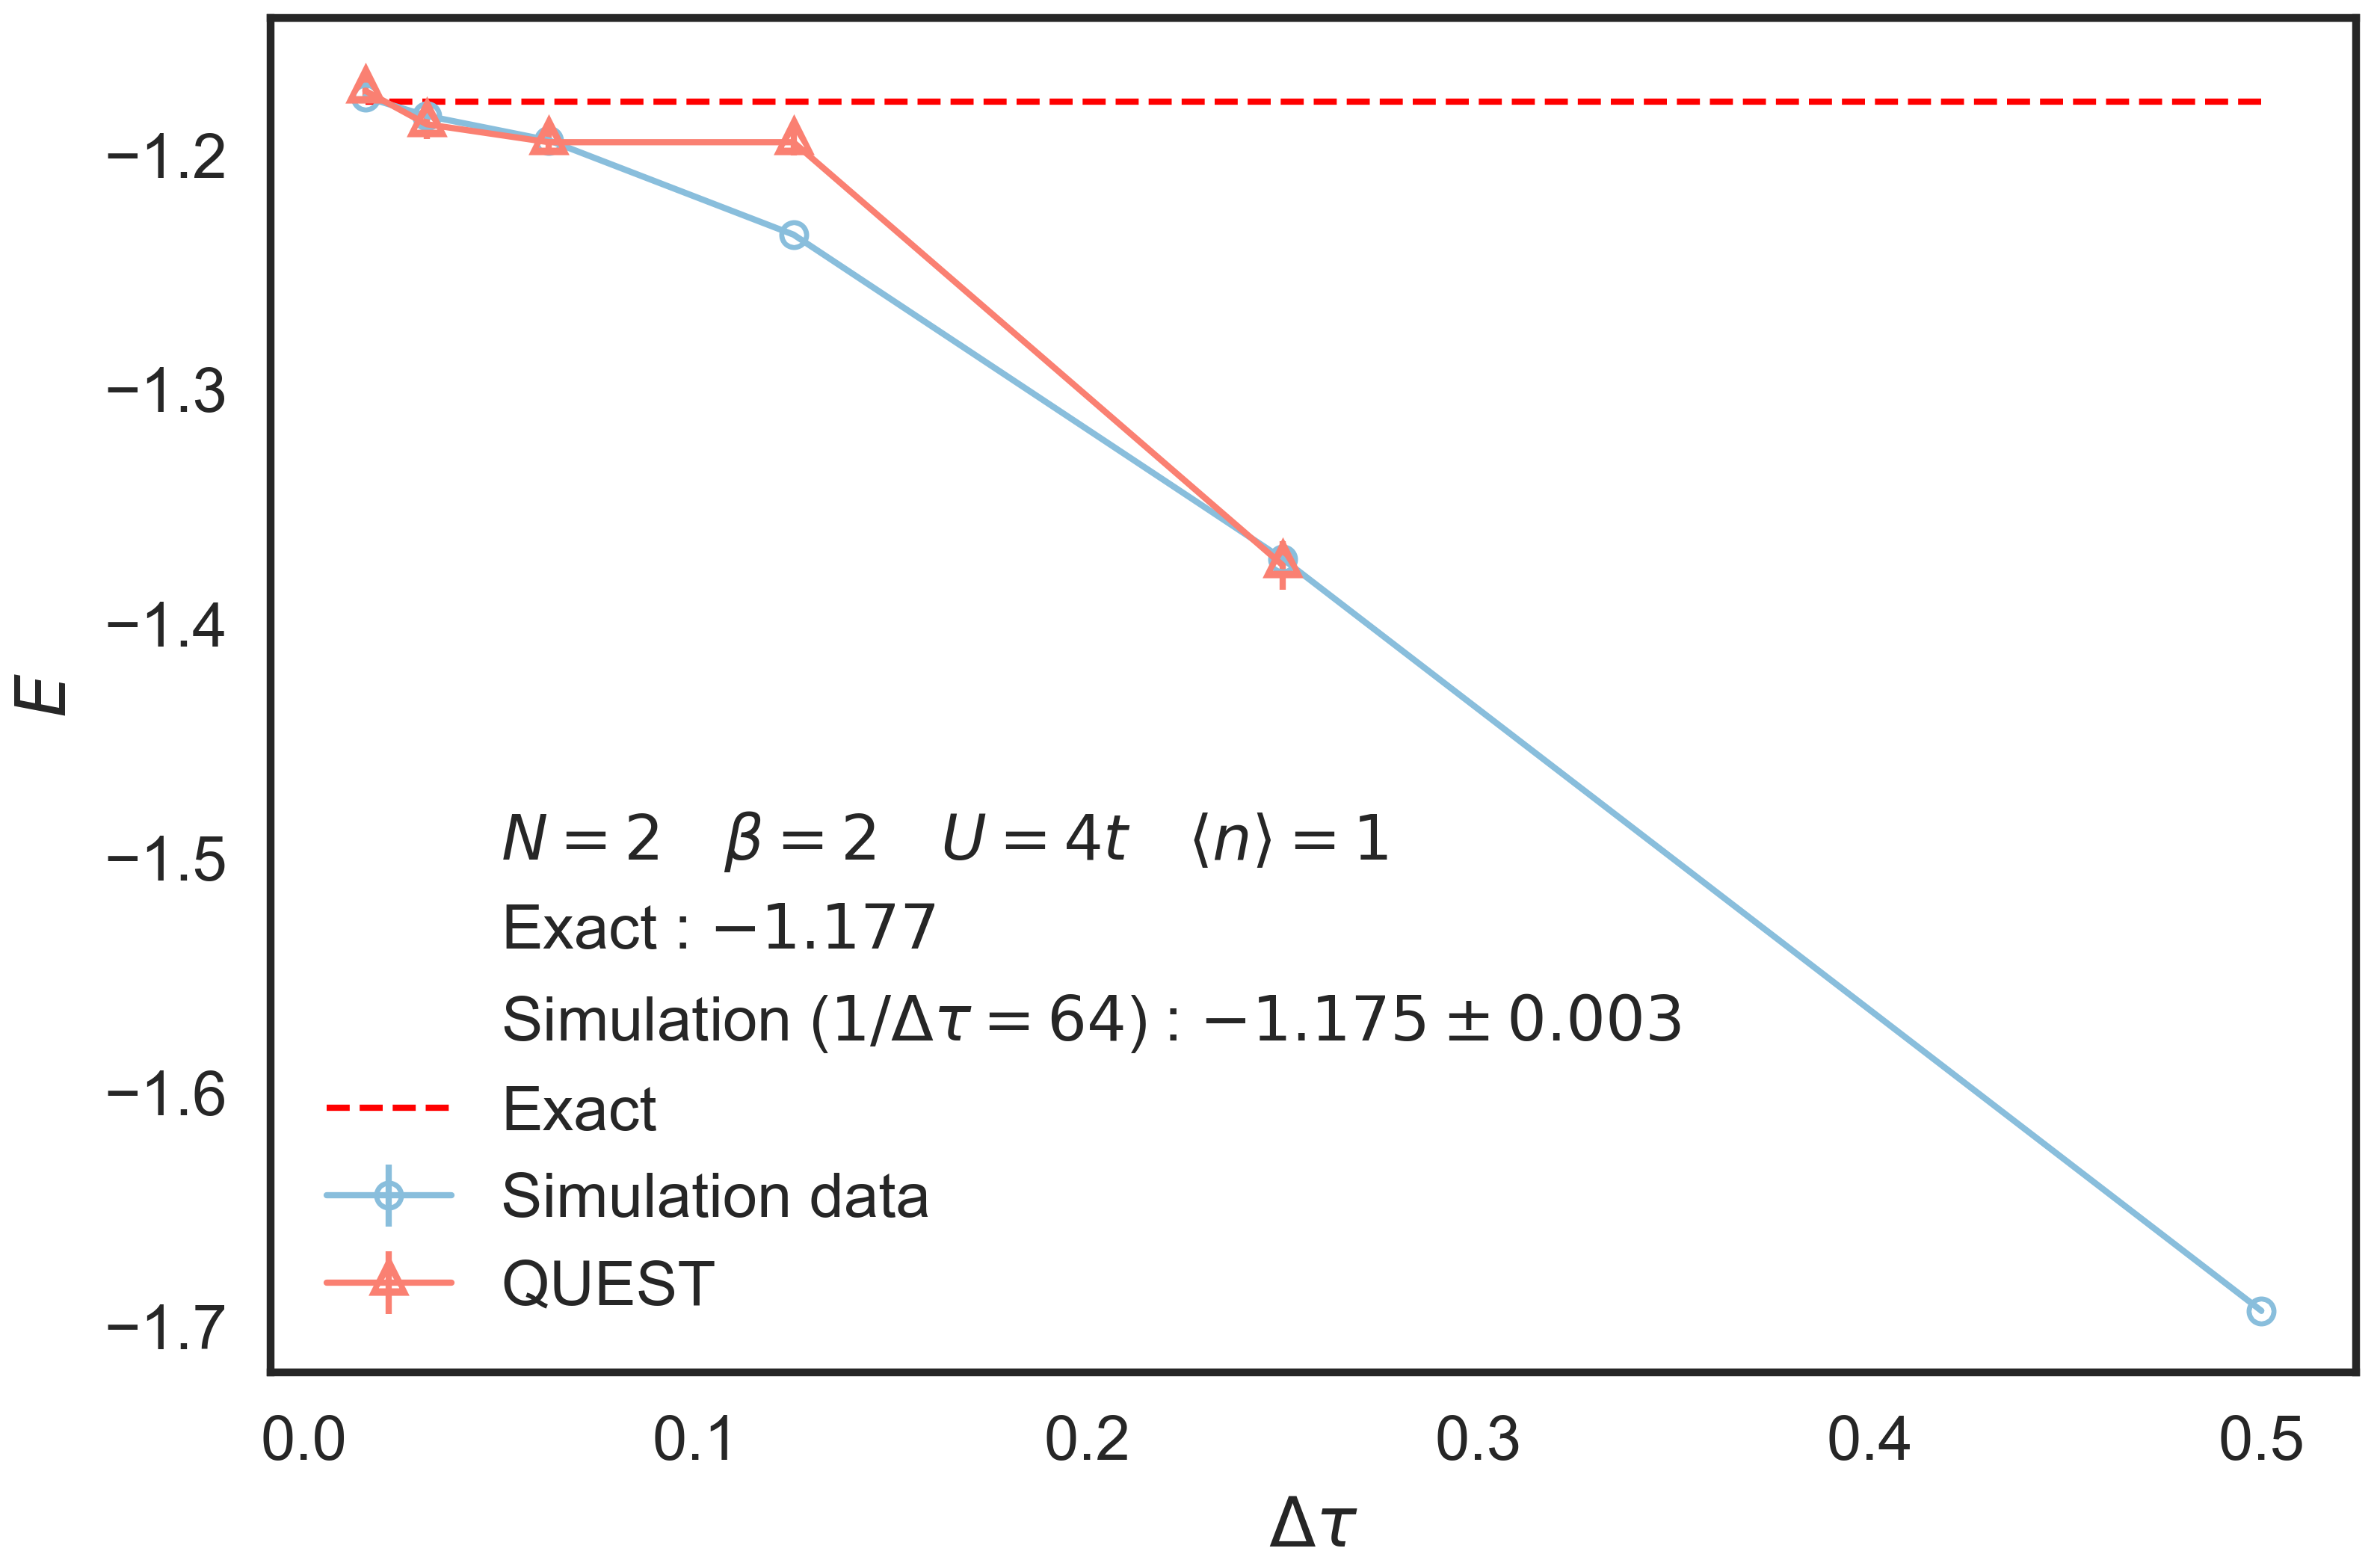
\includegraphics[scale=0.53]{Applications/Ehirsch1982.png}
\hspace{0.3cm}
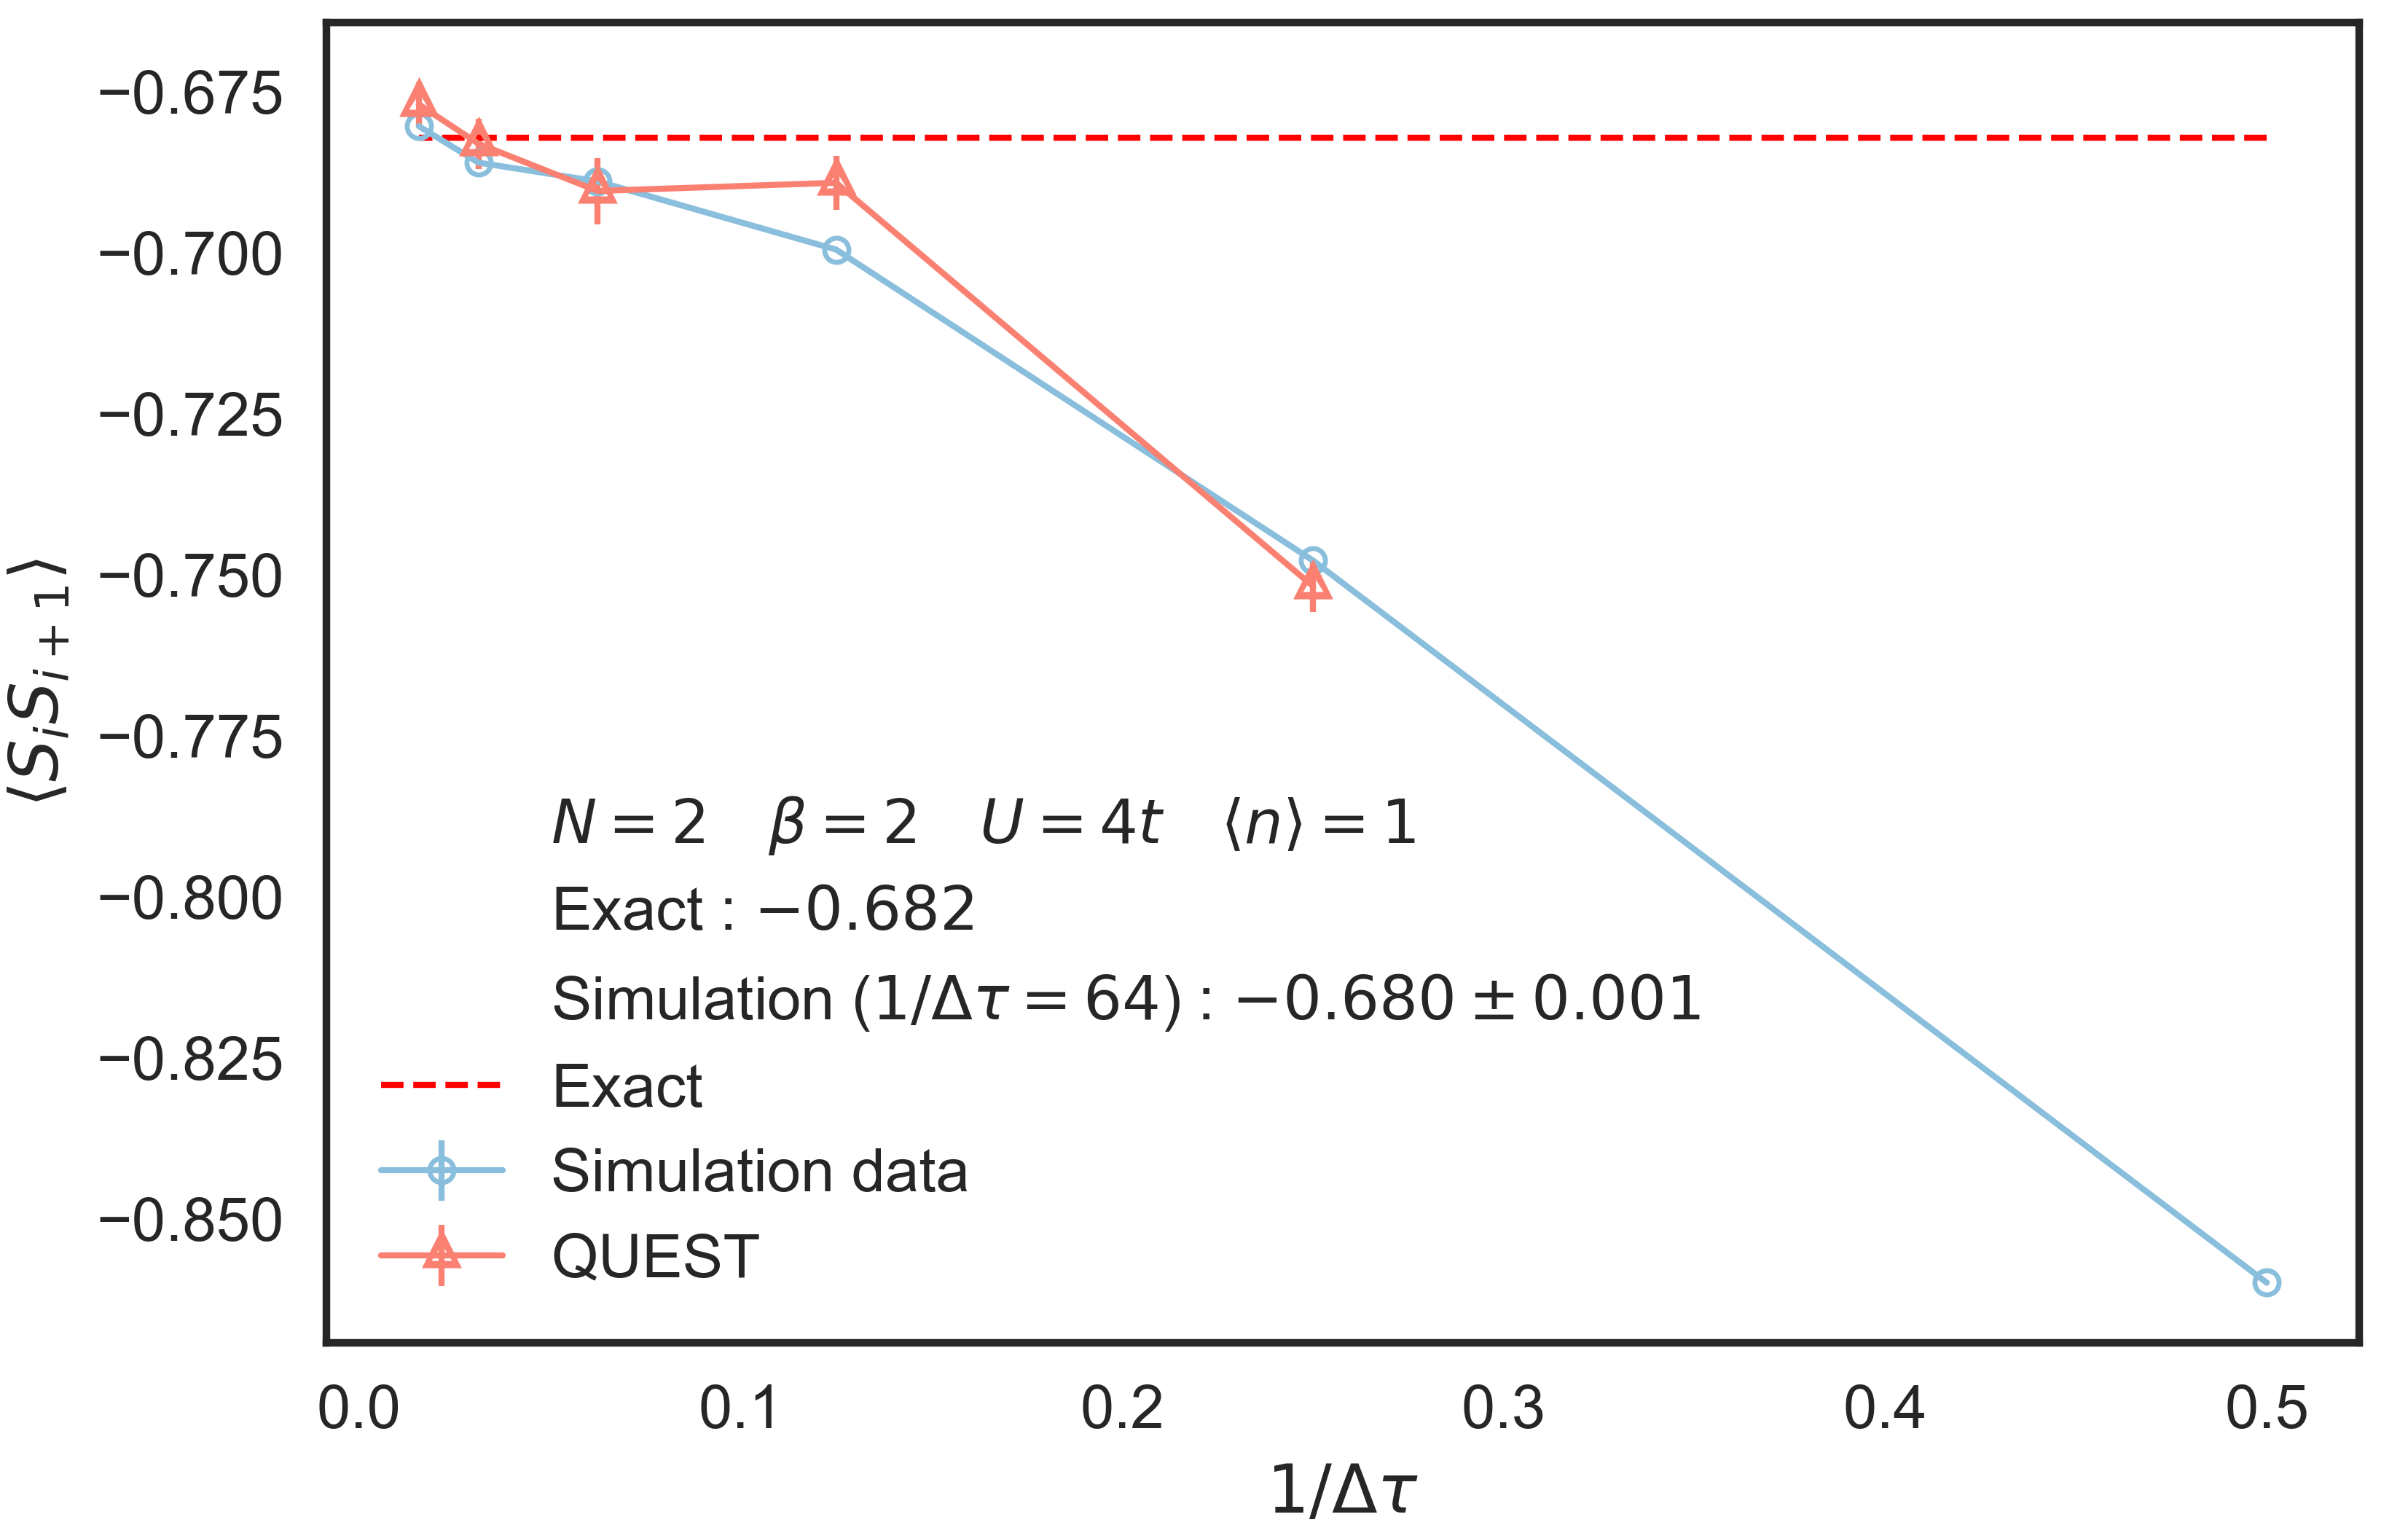
\includegraphics[scale=0.53]{Applications/SiSjhirsch1982.png}
\caption[Convergence of some of the measured observables to the value given by exact diagonalization for $N=2$, $\beta = 2 t$, $U = 4 t$.
Comparison with the results of \texttt{QUEST}.]{Convergence of some of the measured observables (left: total energy; right: spin-spin correlation) to the value given by exact diagonalization for $N=2$, $\beta = 2 t$, $U = 4 t$.
Comparison with the results of \texttt{QUEST}.}
\end{figure}
